\chapter{Menagerie of Wreath-Building Dynamos}
\label{chapter:menagerie of dynamos}
%\chapter{Magnetic Wreathes Appear in Many Dynamos}

In the preceding chapters we have extensively explored the
characteristics of two dynamo solutions.  Those simulations, cases D3
and D5 at three and five times the solar rotation rate, are part of a
much larger family of simulations that we have conducted which explore
the interplay between convection, rotation and magnetism in younger
suns.  In this chapter we present a sampling of simulations rotating
from half the current solar rate to fifteen times the solar rate.
This spans a range of ages for a star like the sun, from just a few
million years after formation when its rotating quite rapidly to a few
billion years older than the current age of the Sun, when our star
will rotate more slowly.  Rotation and age are inextricably linked,
and there are likely to be significant changes in the stellar
structure over these interval of several billion years, as the
luminosity of the star gradually increases, helium settles into the
core and the depth of the convection zone itself shifts.  Here we have neglected 
those changes by retaining a stellar structure appropriate for the
current Sun.  We have instead explored only the effects of faster and
slower rotation, to begin disentangling the varied physical
effects present in real stellar observations.  Future work should
clearly include an exploration of the dual variation of rotation and
structure with age, as in \cite{Ballot_et_al_2007}, but at present
observed stellar ages remain highly imprecise which complicates such efforts.

\clearpage
The parameter space explored by the simulations is summarized in
Tables~\ref{table:pm0.5_dynamos_sim_parameters}-\ref{table:pm0.5_failed_dynamos_sim_parameters}.
Table~\ref{table:pm0.5_dynamos_sim_parameters}
details our successful dynamos at varying levels of
turbulence conducted at a fixed magnetic Prandtl number
$\mathrm{Pm}=0.5$ and fluid Prandtl number $\mathrm{Pr}=0.25$.  
One set of simulations (D3-D15) are
conducted on the familiar parameter path with turbulent diffusivities
scaling as
\begin{equation}
  %\nu = 0.25 \kappa = 0.5 \eta \propto \left(\frac{\Omega_0}{\Omega_\odot}\right)^{-2/3}
  \nu, \kappa, \eta \propto \left(\Omega_0\right)^{-2/3}\thinspace.
  \label{eq:diffusivity scaling}
\end{equation}
Other simulations (D3a, D3b, etc.) sample varying levels of turbulence
at each rotation rate.  At the lower rotation rates 
($\Omega_0 \leq 1.5\thinspace\Omega_\odot$), dynamo action was not
realizable at $\mathrm{Pm}=0.5$ along this main branch of solutions,
but is achieved for more turbulent simulations (D1.5a, D0.5a, etc.).  
Table~\ref{table:high_pm_sim_parameters} details an additional
selection of simulations which were carried out at higher  
magnetic Prandtl numbers ($\mathrm{Pm}=1-4$) for various rotation rates.
Lastly, a selection of failed dynamos are reported in
Table~\ref{table:pm0.5_failed_dynamos_sim_parameters}, to help constrain the
boundaries in parameter space for dynamo action in these simulations.



\begin{deluxetable}{lcccccccccccrc}
\rotatedeluxetable
   \tabletypesize{\footnotesize}
    \tablecolumns{14}
    \tablewidth{0pt}  % `natural' size 
    \tablecaption{Overview of Dynamos at Pm=0.5
    \label{table:pm0.5_dynamos_sim_parameters}}
    \tablehead{\colhead{Case}  &  
      \colhead{$N_r,N_\theta,N_\phi$} &
      \colhead{Ra} &
      \colhead{Ta} &
      \colhead{Re} &
      \colhead{Re$'$} &
      \colhead{Rm} &
      \colhead{Rm$'$} &
      \colhead{Ro} &
      \colhead{Roc} &
      \colhead{$\nu$} &
      \colhead{$\eta$} &
      \colhead{$\Omega_0/\Omega_\sol$} &
      \colhead{Time-dependence}
   }
   \startdata

\sidehead{Dynamos on the $\eta \propto \Omega_0^{-2/3}$ path (denoted in Fig.~\ref{fig:dynamo parameter space} with black triangles)}
  D3    & $ \phn 97 \times  256 \times  512\phn$ &    3.28$ \times 10^{  5}$ &     1.22$ \times 10^{  7}$ & 173 &  104 &   86 &   52 &    0.374 &    0.315 &     1.32 &     2.64 &  3 & S \\
  D5    & $ \phn 97 \times  256 \times  512\phn$ &    1.04$ \times 10^{  6}$ &     6.70$ \times 10^{  7}$ & 268 &  132 &  134 &   66 &    0.272 &    0.241 &    0.940 &     1.88 &  5 & C \\
  D10   & $ \phn 97 \times  512 \times 1024$ &    3.22$ \times 10^{  6}$ &     6.75$ \times 10^{  8}$ & 253 &  228 &  126 &  114 &    0.153 &    0.134 &    0.592 &     1.18 & 10 & C \\
  D15   & $ 129 \times  512 \times 1024$ &    7.05$ \times 10^{  6}$ &     2.61$ \times 10^{  9}$ & 288 &  272 &  144 &  136 &    0.119 &    0.101 &    0.452 &    0.904 & 15 & C \\%[3mm]

\sidehead{Dynamos at other turbulence levels (denoted with colored triangles)}
 D0.5a & $ 145 \times  256 \times  512\phn$ &    2.52$ \times 10^{  4}$ &     2.01$ \times 10^{  5}$ & 154 &  127 &   77 &   63 &     2.45 &    0.688 &     1.72 &     3.43 &  0.5 & S \\
 D0.5b & $ 145 \times  512 \times 1024$ &    1.43$ \times 10^{  4}$ &     8.03$ \times 10^{  5}$ & 395 &  347 &  197 &  173 &     3.29 &    0.779 &    0.859 &     1.72 &  0.5  & O/C? \\[3mm]
  D1.5a & $ \phn 97 \times  256 \times  512\phn$ &    2.33$ \times 10^{  5}$ &     5.02$ \times 10^{  6}$ & 215 &  178 &  107 &   89 &    0.993 &    0.404 &     1.03 &     2.06 &  1 & S \\
  D1.5b & $ 257 \times  512 \times 1024$ &    7.24$ \times 10^{  5}$ &     2.01$ \times 10^{  7}$ & 483 &  414 &  241 &  207 &     1.54 &    0.371 &    0.515 &     1.03 &  1 & O/C? \\[3mm]
  D3a   & $ \phn 97 \times  256 \times  512\phn$ &    5.84$ \times 10^{  5}$ &     2.41$ \times 10^{  7}$ & 244 &  154 &  122 &   77 &    0.447 &    0.295 &    0.940 &     1.88 &  3 & O/C \\
  D3b   & $ 143 \times  512 \times 1024$ &    1.11$ \times 10^{  6}$ &     6.08$ \times 10^{  7}$ & 343 &  273 &  171 &  136 &    0.566 &    0.257 &    0.592 &     1.18 &  3 & C \\[3mm]
  D10 L & $ \phn 97 \times  512 \times 1024$ &    2.15$ \times 10^{  6}$ &     2.68$ \times 10^{  8}$ & 331 &  110 &  165 &   55 &    0.131 &    0.177 &    0.940 &     1.88 &  10 & C \\

 \enddata
 \vskip-0.75cm %this actually works!  BPB 7/26/09
 \tablecomments{Dynamo simulations at many different rotation rates.
        All simulations have inner radius 
	$r_\mathrm{bot} = 5.0 \times 10^{10}$cm and outer radius of 
        $r_\mathrm{top} = 6.72 \times 10^{10}$cm, with 
	$L = (r_\mathrm{top}-r_\mathrm{bot}) = 1.72 \times 10^{10}$cm
	the thickness of the spherical shell.
	%
	All quantities are the same as defined in Table~\ref{table:dynamo_sim_parameters}.  
	%
	Briefly recapping, evaluated at mid-depth are the
	Rayleigh number $\mathrm{Ra}$, 
	the Taylor number $\mathrm{Ta}$, 
	the rms Reynolds number $\mathrm{Re}$ and
	fluctuating Reynolds number $\mathrm{Re}'$,
	the magnetic Reynolds number $\mathrm{Rm}$ 
	and fluctuating magnetic Reynolds number 
        $\mathrm{Rm}'$, 
	the Rossby number $\mathrm{Ro}$ ,
	and the convective Rossby number 
	$\mathrm{Roc}$.
	For all simulations, the Prandtl number $\mathrm{Pr} = \nu / \kappa$ is 0.25 
	and the magnetic Prandtl number $\mathrm{Pm}=\nu/\eta$ is 0.5.  
	The viscous and magnetic diffusivity, $\nu$ and $\eta$, are
	quoted at mid-depth (in units of $10^{12}~\mathrm{cm}^2\mathrm{s}^{-1}$).
        The rotation rate $\Omega_0$ of each reference frame is in multiples
        of the solar rate $\Omega_\sol=2.6 \times 10^{-6}~\mathrm{rad}\:\mathrm{s}^{-1}$ or $414$ nHz.  
        The~viscous time scale at mid-depth $\tau_\nu = L^2/\nu$ is
        $3640$~days for case D5 and the resistive time scale is $1820$~days.
	Rotation periods at three and five times the solar rate are in
	turn 9.3~days and 5.6~days.  The time-dependence of the dynamo
	is indicated, with dynamos that build persistent and steady wreaths
	labeled by \emph{S}, dynamos where the energies oscillate
        significantly by \emph{O},
	and dynamos that achieve cycles of polarity reversal by \emph{C}.  
	These cases are denoted in Figure~\ref{fig:dynamo
        parameter space} with triangles.
	}
\end{deluxetable}

\begin{deluxetable}{lccccccccccccrc}
\rotatedeluxetable
   \tabletypesize{\footnotesize}
    \tablecolumns{15}
    \tablewidth{0pt}  % `natural' size 
    \tablecaption{Dynamos at Higher Pm
    \label{table:high_pm_sim_parameters}}
    \tablehead{\colhead{Case}  &  
      \colhead{$N_r,N_\theta,N_\phi$} &
      \colhead{Ra} &
      \colhead{Ta} &
      \colhead{Re} &
      \colhead{Re$'$} &
      \colhead{Rm} &
      \colhead{Rm$'$} &
      \colhead{Ro} &
      \colhead{Roc} &
      \colhead{$\nu$} &
      \colhead{$\eta$} &
      \colhead{$\mathrm{Pm}$} &
      \colhead{$\Omega_0/\Omega_\sol$} &
      \colhead{Time-dependence}
   }
   \startdata
             M3 & $ 129 \times  512 \times 1024$ &    7.18$ \times 10^{  4}$ &     1.25$ \times 10^{  6}$ & 179 &  125 &  716 &  500 &     1.04 &    0.656 &     1.37 &    0.343 &  4 & 1 & O/C?\\
        M3-pcpf & $ 129 \times  512 \times 1024$ &    7.31$ \times 10^{  4}$ &     1.25$ \times 10^{  6}$ & 162 &  123 &  651 &  492 &     1.01 &    0.663 &     1.37 &    0.343 &  4 & 1 & C \\[3mm]

  D1.25a-pm2 & $ 145 \times  256 \times  512\phn$ &    1.72$ \times 10^{  5}$ &     3.48$ \times 10^{  6}$ & 238 &  211 &  476 &  422 &    1.29 &    0.419 &     1.03 &    0.52 &  2 & 1.25 & O? \\[3mm]

  D3-pm1 & $ 145 \times  256 \times  512\phn$ &    2.98$ \times 10^{  5}$ &     1.22$ \times 10^{  7}$ & 149 &  102 &  149 &  102 &    0.372 &    0.300 &     1.32 &     1.32 &  1 & 3 & C \\
  D3-pm2 & $ 145 \times  512 \times 1024$ &    3.08$ \times 10^{  5}$ &     1.22$ \times 10^{  7}$ & 145 &  101 &  291 &  202 &    0.370 &    0.306 &     1.32 &    0.660 &  2 & 3 & C \\
  D3-pm4 & $ 145 \times  512 \times 1024$ &    3.12$ \times 10^{  5}$ & 1.22$ \times 10^{  7}$ & 161 &   94 &  644 &  377 &    0.336 & 0.308 &     1.32 &    0.330 &  4& 3 & C? \\[3mm]

  D5-pm1 & $  97 \times  256 \times  512$ &    8.24$ \times 10^{  5}$ &     6.70$ \times 10^{  7}$ & 180 &  132 &  180 &  132 &    0.241 &    0.214 &    0.940 &    0.940 &  1 & 5 & C \\

   \enddata
 \tablecomments{Parameters are defined in Table~\ref{table:pm0.5_dynamos_sim_parameters}.
 The dynamos shown in this table
 are at relatively high magnetic Prandtl numbers, with
 $\mathrm{Pm}=1-4$.  These cases are denoted in Fig.~\ref{fig:dynamo
 parameter space} with diamonds.  Case~M3 was initially published in
 \cite{Brun_et_al_2004} and has been continued here for comparison.
 Cases~M3 and M3-pcpf are at Prandtl number $\mathrm{Pr}=0.125$,
 rather than $\mathrm{Pr}=0.25$ as in the other simulations of this thesis.
 Case~D1.25a-pm2 has been run to help constrain the boundary of
 sustained dynamo action and has currently only evolved for 1000~days.}
\end{deluxetable}


\begin{deluxetable}{lccccccccccccr}
\rotatedeluxetable
   \tabletypesize{\footnotesize}
    \tablecolumns{14}
    \tablewidth{0pt}  % `natural' size 
    \tablecaption{Dynamos That Failed
    \label{table:pm0.5_failed_dynamos_sim_parameters}}
    \tablehead{\colhead{Case}  &  
      \colhead{$N_r,N_\theta,N_\phi$} &
      \colhead{Ra} &
      \colhead{Ta} &
      \colhead{Re} &
      \colhead{Re$'$} &
      \colhead{Rm} &
      \colhead{Rm$'$} &
      \colhead{Ro} &
      \colhead{Roc} &
      \colhead{$\nu$} &
      \colhead{$\eta$} &
      \colhead{$\mathrm{Pm}$} &
      \colhead{$\Omega_0/\Omega_\sol$}
   }
   \startdata
  D1a     & $ \phn 97 \times  256 \times  512\phn$ &    5.67$ \times 10^{  4}$ &     8.03$ \times 10^{  5}$ & 138 &  118 &   69 &   59 &     1.22 &    0.494 &     1.72 &     3.43 & 0.5& 1 \\
  D1a-pm1 & $  \phn 97 \times  256 \times  512\phn$ &    5.66$ \times 10^{  4}$ &     8.03$ \times 10^{  5}$ & 140 &  118 &  140 &  118 &     1.22 &    0.493 &     1.72 &     1.72 &  \phn1&1 \\
  D1a-pm2 & $  \phn 97 \times  512 \times 1024$ &    5.23$ \times 10^{  4}$ &     8.03$ \times 10^{  5}$ & 139 &  121 &  279 &  243 &     1.23 &    0.475 &     1.72 &    0.859 &  \phn2&1 \\
  D1b     & $  \phn 97 \times  256 \times  512\phn$ &    1.22$ \times 10^{  5}$ &     2.23$ \times 10^{  6}$ & 220 &  212 &  110 &  106 &     1.65 &    0.444 &     1.03 &     2.06 & 0.5& 1 \\
  D1b-pm1 & $  \phn 97 \times  256 \times  512\phn$ &    1.23$ \times 10^{  5}$ &     2.23$ \times 10^{  6}$ & 224 &  212 &  224 &  212 &     1.64 &    0.447 &     1.03 &     1.03 & \phn1& 1 \\[3mm]

  D1.25a & $ 145 \times  256 \times  512\phn$ & 1.72$ \times 10^{ 5}$ & 3.48$ \times 10^{  6}$ & 238 &  211 &  119 &  106 &  1.29 &    0.419 &     1.03 &    2.06 &  0.5 & 1.25\\
  D1.25a-pm1 & $ 145 \times 256 \times 512\phn$ & 1.72$ \times 10^{  5}$ & 3.48$ \times 10^{  6}$ & 238 &  211 &  238 &  211 &    1.29 &    0.419 &     1.03 &    1.03 &  1 & 1.25  \\[3mm]

  D1.5  & $ 145 \times  256 \times  512\phn$ &    8.73$ \times 10^{  4}$ & 1.21$ \times 10^{  6}$ & 137 &   74 &   68 &   37 &    0.682 & 0.516 &     2.10 &     4.19 &  0.5 & 1 \\
  D3 L  & $  \phn 97 \times  256 \times  512 \phn$ &    1.21$ \times 10^{  5}$ &     2.82$ \times 10^{  6}$ & 109 &   41 &   54 &   20 &    0.279 &    0.409 &     2.75 &     5.50 & 0.5& 3 \\[3mm]

 \enddata
 \tablecomments{These simulations failed to
 attain substantial dynamo action.  Some are marginal, with very low
 magnetic energies, but in most cases the magnetic energies decline
 exponentially.   These cases are denoted in Fig.~\ref{fig:dynamo
 parameter space} with crosses and are labeled \emph{F}.}
\end{deluxetable}



The parameter space explored by this family of dynamo solutions is 
illustrated in Figure~\ref{fig:dynamo parameter space}.  Here the primary input
parameters of our dynamo simulations, the turbulent diffusivity $\eta$
and the bulk rotation rate $\Omega_0$, are shown for all of our
convection zone dynamos.  As detailed in the tables, triangles denote
dynamos with $\mathrm{Pm}=0.5$ while diamonds denote high
$\mathrm{Pm}$ dynamos.  The failed dynamos are shown with blue
crosses.  As becomes immediately apparent, near the solar rotation
rate there appears to be a deep dip in this parameter space where
successful dynamos can occur, and such dynamos must be run at
substantially lower diffusivities.  A few dynamos are
labeled with case names in Figure~\ref{fig:dynamo parameter space} for
reference with the tables.  

\begin{figure}[!t]
  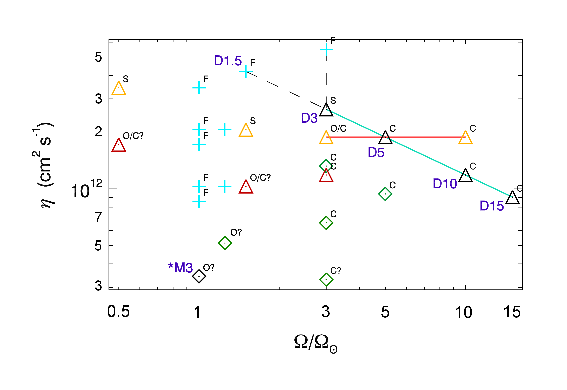
\includegraphics[width=\linewidth]{figs/chapter_8/apj_dynamo_eta_paths.eps}
  \caption[Map of full dynamo $\eta-\Omega_0$ parameter space]
  {Map of full dynamo $\eta-\Omega_0$ parameter space.  
  These parameters are the eddy diffusivity $\eta$ and bulk
  rotation rate $\Omega_0$. 
  Solutions at magnetic Prandtl number 0.5 are shown with triangles
  while cases at higher magnetic Prandtl numbers are shown with
  diamonds.  Cases that build
  steady, persistent magnetic wreaths are labeled \emph{S}, while
  those that undergo oscillations but rarely flip polarities are
  \emph{O} and those that undergo many polarity reversals are 
  \emph{C}.  Cases shown with blue crosses and labeled \emph{F} are
  failed dynamos, where magnetic energies drop over long periods of
  time.  Question marks indicate where the time-dependence remains
  uncertain.  
  See~Tables~\ref{table:pm0.5_dynamos_sim_parameters}~(triangle
  symbols), \ref{table:high_pm_sim_parameters}~(diamonds) and
  \ref{table:pm0.5_failed_dynamos_sim_parameters}~(crosses) 
  for simulation details.
  \label{fig:dynamo parameter space}}
\end{figure}


All dynamos shown in Figure~\ref{fig:dynamo parameter space} build
large-scale magnetic wreaths in the bulk of their convection zone.
The character of the wreaths changes somewhat
across this parameter space.  Generally, magnetic wreaths in the
rapidly rotating simulations $(\Omega_0 \gtrsim 3\thinspace \Omega_\odot)$ fill the
bulk of the convection zone, with substantial structure in both radius
and latitude, as seen previously in cases D3 and D5
(Chapters~\ref{chapter:case D3}-\ref{chapter:dynamo production}). 
The mean poloidal field is typically complex, with generally two
different polarities in the polar and equatorial regions.  These wreaths
can also be single structures that cross the equator and primarily
have a single polarity, as will be seen for the most rapidly rotating
cases D10 and D15.  In the more slowly rotating cases $(\Omega_0 \lesssim
1.5 \thinspace\Omega_\odot)$, the wreaths become increasingly confined to the
bottom of the convection zone, and while they retain their latitudinal
extent, much of the prominent radial structure seen in the rapidly
rotating cases disappears.  At present it is unclear whether this is a
matter of more effective turbulent pumping in those simulations, or
changes in the differential rotation and the velocity shear available
for amplifying the magnetic fields.  The mean poloidal field in
these slower rotating simulations is often of a single polarity
throughout the convection zone.

Many of the dynamos in Figure~\ref{fig:dynamo parameter space}
exhibit temporal variations, with either
oscillations in magnetic energies or cycles of activity where the
polarity of the global-scale magnetic fields routinely changes.  The
labeling denotes the temporal characteristics of the dynamo
solution, with steady solutions that do not oscillate noticeably
indicated by \emph{S}, solutions that oscillate frequently but rarely change
their global-scale polarity by \emph{O/C}, and solutions that routinely
interchange polarities by \emph{C}.  

Overall, we have found three solutions that are steady in nature
(cases~D0.5a, D1.5a, and D3), and these generally appear to cluster
near the boundary in parameter space between successful dynamos and
failed dynamos that do not successfully regenerate their magnetic
fields.  Even these steady simulations evince small oscillations in
their volume-averaged magnetic energy densities, as seen previously in
case~D3 (Chapter~\ref{chapter:case D3}).  As the magnetic Reynolds
number increases, the flows and magnetic fields tend to become more
time-dependent, with the dynamos showing either large oscillations in
their magnetic energies or undergoing repeated global-scale magnetic
polarity reversals. 

We begin by returning to familiar ground, exploring
with more extensive sampling the turbulent parameter space in a
series of simulations rotating three times faster than the Sun.
We first examine the onset of time-dependent behavior in simulations
at three times the current solar rate.


\section{Higher Levels of Turbulence at  $3\thinspace\Omega_\odot$ and $\mathrm{Pm}=0.5$}
In our simulations rotating at three times the solar rate, we have
examined how our wreaths of magnetism change as we raise the overall
level of turbulence.  This is accomplished along one of two paths in
parameter space.  On the first
path, we simultaneously decrease $\nu, \kappa$ and $\eta$, thus maintaining
a fluid Prandtl number of 0.25 and magnetic Prandtl number of 0.5 as
the diffusivities are decreased.  This path corresponds to dynamo
cases D3, D3a and D3b.  On this path the convection becomes more
complex and turbulent and in hydrodynamic simulations would drive a
substantially stronger differential rotation.  Both the fluid Reynolds
number and the magnetic Reynolds number increase in the successively
more turbulent simulations. 
In these dynamo solutions we find that wreaths of magnetism persist but begin
to undergo oscillations similar to those found in case~D5 rotating at
five times the solar rate.   

\textbf{Case~D3a --} The time-dependence of case~D3a is shown in Figure~\ref{fig:D3a}.
This simulation is somewhat more turbulent than case~D3, with typical
rms and fluctuating Reynolds numbers of 244 and 154 respectively, and
rms and fluctuating magnetic Reynolds numbers of 122 and 77.
Case~D3a undergoes many oscillations in energy and mean field strength
with a typical timescale of 500 days, as shown in the time traces of
Figure~\ref{fig:D3a}$a,b$.  Generally, the azimuthally averaged
toroidal and poloidal fields are stable, retaining the same polarity
through many such oscillations.  Only very rarely 
(twice in the 16000 days shown here) do the global-scale fields flip
in polarity.  This is evident in time-latitude plots of
$\langle B_\phi \rangle$ at mid-convection zone, shown in
Figure~\ref{fig:D3a}$c$.  Here we note that the large excursion in
mean field strengths occurring between days 13000-14500 corresponds to
a strong, single polarity state.  As in case~D5 during similar
excursions, we find that during this interval of time the mean poloidal
field has changed from an odd-parity state, with strong contributions
from the odd-$\ell$ components, to an even-parity state where the
even-$\ell$ components are more prominent.  The dynamo exits this
state at roughly day 14500 and appears to return to a more normal
state, with two opposite polarity wreaths and a predominantly
odd-parity poloidal field.  

\begin{figure*}[!p]
  \begin{center}
    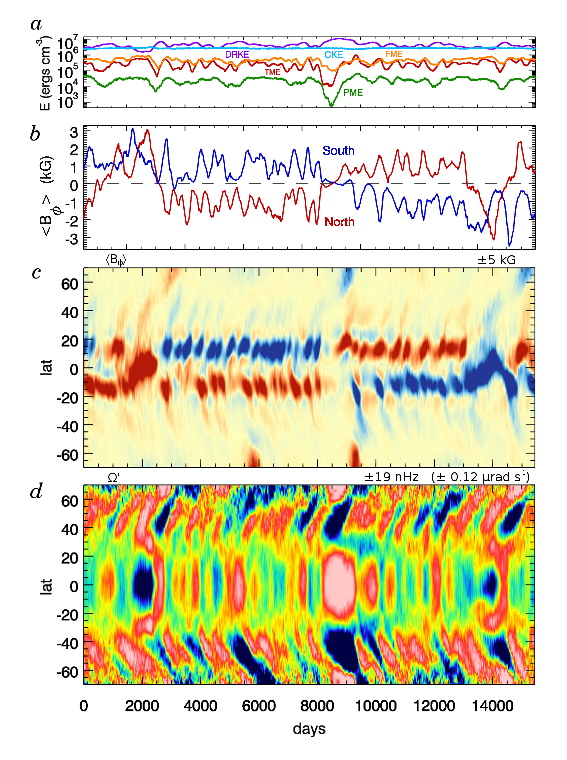
\includegraphics[width=0.8\linewidth]{figs/chapter_8/time_history_mmc_vturf_3_SC.eps}
%    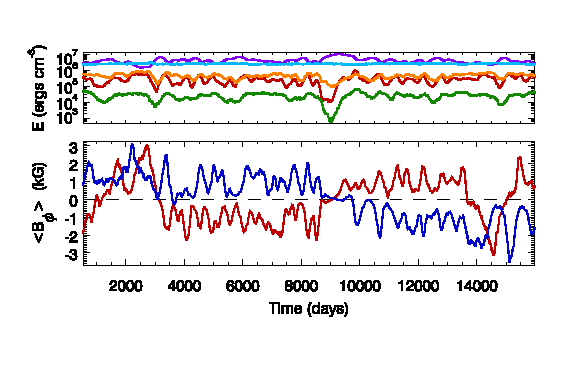
\includegraphics[width=\linewidth]{figs/chapter_8/apj_dynamo_reversal_mmc_vturf_3_SC_Bp-avg-trace-0.85R.eps}\\
%    \hskip-1.5cm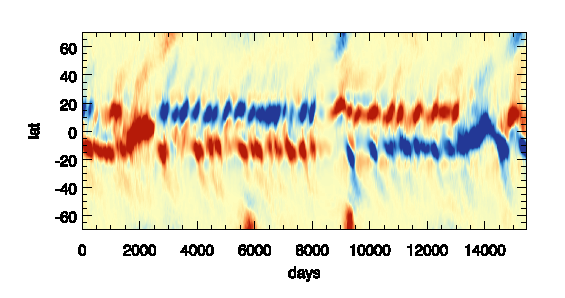
\includegraphics[width=1.1\linewidth]{figs/chapter_8/azav_mmc_vturf_3_SC_4000_11810_Bp-avg-trace-0.85R.eps}\\
%    \hskip-1.5cm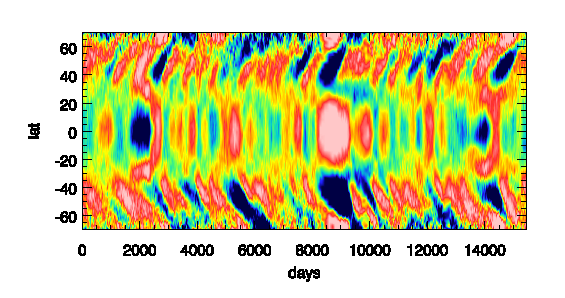
\includegraphics[width=1.1\linewidth]{figs/chapter_8/azav_mmc_vturf_3_SC_4000_11810_Vp-timelat-cube_flucOmega.eps}
  \end{center}
  \caption[Time-dependent behavior in the oscillating case~D3a]
	  {Time-dependent behavior in the oscillating case~D3a.  
            $(a)$~Volume-averaged kinetic and magnetic energies, showing DRKE,
	  CKE, TME, PME and FME as labeled.  Many small oscillations
	  occur on roughly 500~day timescales, with a large excursion
	  around day~9000.  
	  $(b)$ Mean $\langle B_\phi \rangle$ averaged over northern
	  and southern hemispheres at mid-convection zone.  Despite
	  the many oscillations, a global-scale polarity reversal occurs
	  only once (near day 9000), with a second significant
	  excursion between roughly days 13000-14500.
	  $(c)$  Time-latitude maps of $\langle B_\phi \rangle$ at
	  mid-convection zone.  During roughly days 13000-14500 a strange,
	  single-polarity state emerges.	  
	  $(d)$ Time-latitude map of $\Omega'$ at mid-convection zone,
	  with time average removed to emphasize the poleward
	  propagating velocity structures. 
	  \label{fig:D3a}}
\end{figure*}

Throughout the history of this case, weak magnetic structures appear
to propagate from the equatorial regions to both poles.  As in case~D5
(Chapter~\ref{chapter:case D5}), these magnetic structures are
associated with local bands of slightly faster differential rotation
which also propagate toward the poles (Fig.~\ref{fig:D3a}$d$).  
These structures are observed
with each oscillation, being launched from the equatorial regions
roughly every 500~days.  At a few intervals in the simulation, very strong
magnetic features appear near the poles (i.e. near days 5500-6000 and
9000-9500).  At present it is unclear whether these are formed through
local amplification of $\langle B_\phi \rangle$ by either the turbulence or the
differential rotation, or if they represent a geometric amplification
of magnetic field as particularly strong wreaths slip to the poles
and are concentrated into a smaller volume there.  These polar
magnetic structures are associated with strong velocity structures.


\begin{figure}
  \begin{center}
    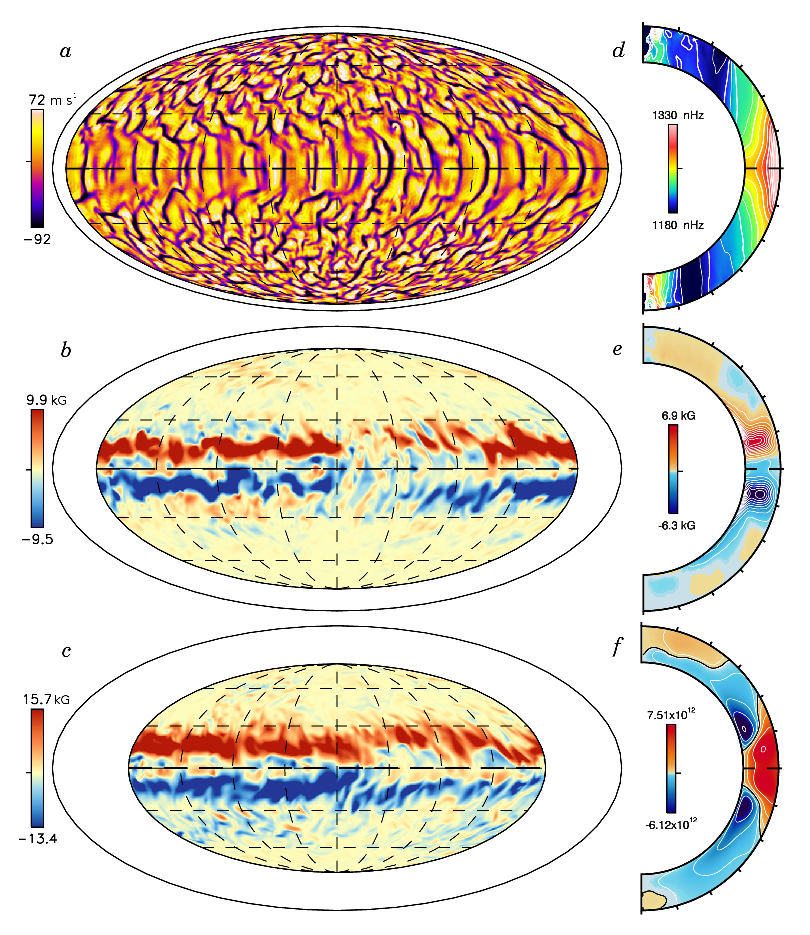
\includegraphics{figs/chapter_8/mmc_vturf_3_SC_patterns.eps}
%    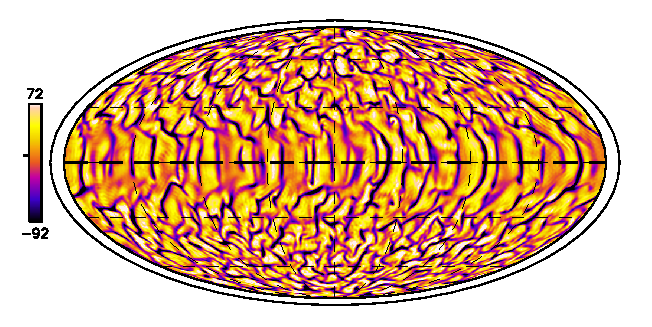
\includegraphics{figs/chapter_8/pub_mmc_vturf_3_SC_shsl_9520_shell0_Vr.eps}
%    
\includegraphics{figs/chapter_8/pub_mmc_vturf_3_SC_9500_9590_Vp.eps}\\
%    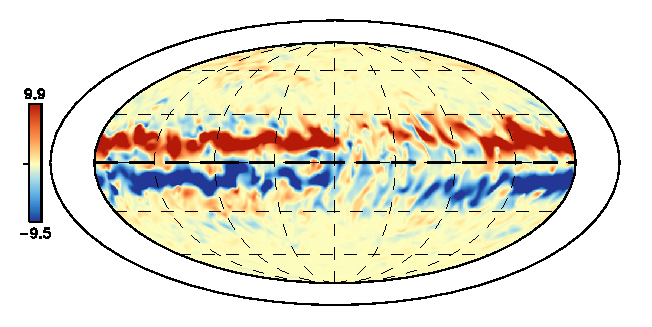
\includegraphics{figs/chapter_8/pub_mmc_vturf_3_SC_shsl_9520_shell1_Bp.eps}
%    
\includegraphics{figs/chapter_8/pub_mmc_vturf_3_SC_9500_9590_Bp.eps}\\
%    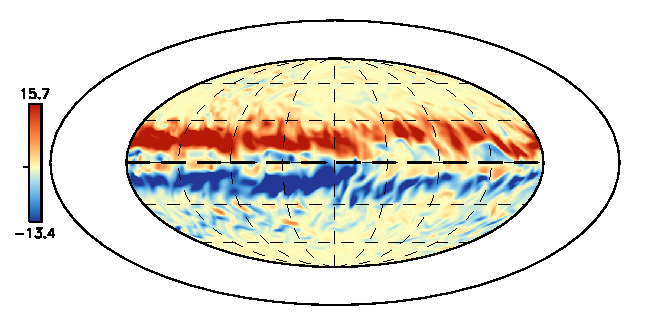
\includegraphics{figs/chapter_8/pub_mmc_vturf_3_SC_shsl_9520_shell2_Bp.eps}
%    
\includegraphics{figs/chapter_8/pub_mmc_vturf_3_SC_9500_9590_Bstream.eps}
  \end{center}
  \caption[Patterns of convection in case D3a]{Patterns of convection
  in case D3a.  $(a)$~Radial velocity $v_r$ in Mollweide projection
  near the top of the shell ($0.95\thinspace R_\odot$).  
  $(b)$~Toroidal magnetic field $B_\phi$ at mid-convection zone
  ($0.85\thinspace R_\odot$) and
  $(c)$~near the bottom of the
  convective shell ($0.73\thinspace R_\odot$).
  These snapshots are shown at day~12200, a time when the mean
  magnetic fields are strong.
  Also shown are 100 day averaged profiles of $(d)$~angular velocity $\Omega$, with fast equator and
  slow poles, $(e)$~mean toroidal field $\langle B_\phi \rangle$ and
  $(f)$~mean poloidal vector potential $\langle A_\phi \rangle$ with
  contours representing the mean poloidal field lines.
  \label{fig:D3a convection}} 
\end{figure}

The patterns of convection achieved in case~D3a are shown in
Figure~\ref{fig:D3a convection}.  The convective cells are a little
more complex than in case~D3 (compare with
Fig.~\ref{fig:case_D3_many_depths}) and the amplitude of the motions
is  10\% faster than in that case.  The toroidal field in this more
turbulent case is somewhat higher, with typical field strengths at
mid-convection zone of almost $\pm10$~kG and peak field strengths of roughly $\pm35$~kG.  In
comparison, typical field strengths in case~D3 were $\pm7$~kG with
peak strengths of roughly $\pm 26$~kG.  This snapshot is taken at an
instant when the mean toroidal fields are quite strong (TME is at a
peak). As such, the magnetic wreaths are
visibly dominated by the mean toroidal field $\langle B_\phi
\rangle$ and their structure appears quite similar to those found in
case~D3.  When the fields are weaker (say at day~12500 when TME and
PME are at a minimum), the structure of the wreaths is very similar,
though their typical field strengths at mid-convection zone are then
only $\pm 5$~kG, with peak field strengths of $\pm 20$~kG.  Thus at
the times when $\langle B_\phi \rangle$ is weak, case~D3a returns to
a state very similar to case~D3.
When case~D3a is in a single-polarity state, between days 13000-14500,
the magnetic fields at mid-convection zone tend to be in a single
wreath of negative polarity that wanders across the equator.
Surrounding this structure is weaker positive polarity field.  

The differential rotation in this case is similar to that
realized in the less turbulent case~D3.  As shown in
Figure~\ref{fig:D3a convection}$d$, the equator remains fast
and prograde while the poles are filled with retrograde flow.
There is substantial radial shear near the equator.  The mean toroidal
field associated with the wreaths of magnetism 
(Fig.~\ref{fig:D3a convection}$e$) is comparable in strength to the fields achieved in
case~D3, but the cores of the wreaths are located slightly closer to
the equator than in case~D3 where they straddled $\pm 15^\circ$.  The
poloidal vector potential (Fig.~\ref{fig:D3a convection}$f$) is also
similar in morphology, though now the equatorial region is comparable
in strength to the poleward regions.  In case~D3, the vector potential
near the equator was about a factor of three weaker than that found in
this case above latitude $\pm15^\circ$.


\textbf{Case~D3b --} When the level of turbulence is increased further (case~D3b,
Fig.~\ref{fig:D3b}$a$-$d$), the global scale fields appear to flip far
more frequently.  This simulation is yet more turbulent, with typical
rms and fluctuating Reynolds numbers of 343 and 273 respectively, and
rms and fluctuating magnetic Reynolds numbers of 171 and 136.
Though this simulation has not achieved nearly as
much time evolution, with 3300 days of total evolution since the
last adjustment of diffusivities, the global scale fields have already
exchanged polarity at least once.  We thus suspect
that these oscillations are due to the higher magnetic Reynolds number
achieved rather than being linked intrinsically to the higher rotation
rate used in D5.  At times, the magnetic wreaths survive for long
intervals, with one pair existing from roughly day~1400 to day~2100.
At other periods, strong wreaths are built in each hemisphere but
only survive for short periods of time, disappearing within a few
hundred days.  This behavior holds true at deeper locations within the
convection zone as well.  After day~2700, wreath building occurs
predominantly in only the southern hemisphere.  As in the other
simulations, prominent velocity structures are launched toward the
polar regions.  In the interval of simulated time, only a few such
structures have appeared, with possibly two in the northern hemisphere
and one in the southern.

\begin{figure*}
  \begin{center}
    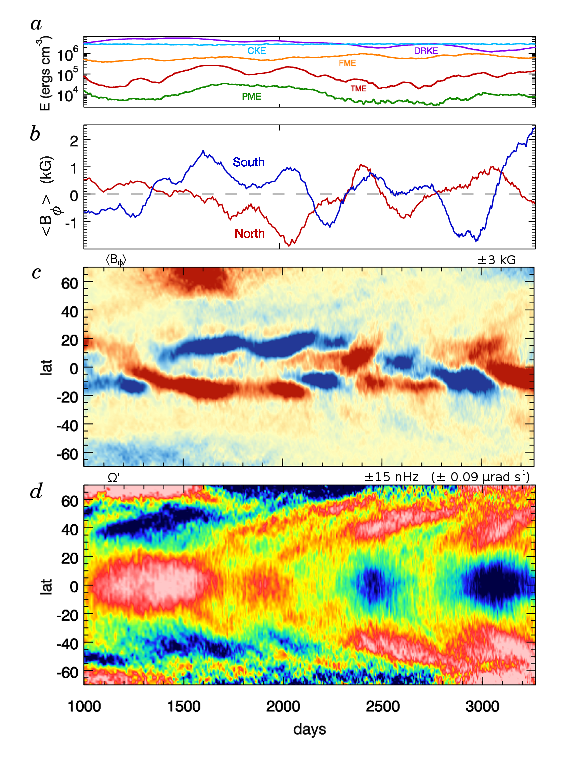
\includegraphics[width=0.8\linewidth]{figs/chapter_8/time_history_mmc_vturf_3_SC2.eps}
%    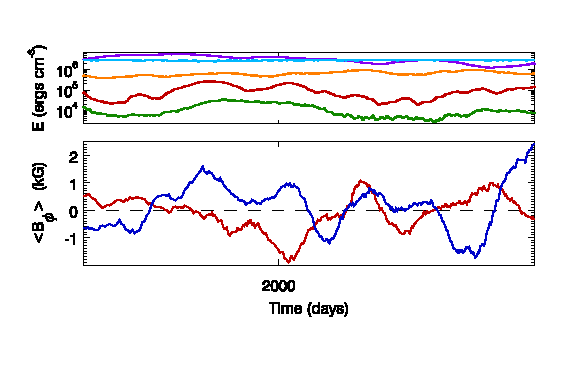
\includegraphics{figs/chapter_8/apj_dynamo_reversal_mmc_vturf_3_SC2_Bp-avg-trace-0.85R.eps}\\
%    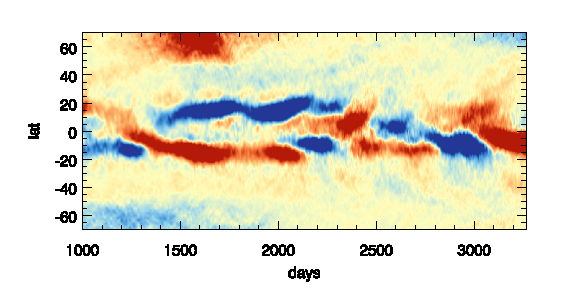
\includegraphics{figs/chapter_8/azav_mmc_vturf_3_SC2_12070_16700_Bp-timelat-cube.eps}\\
%    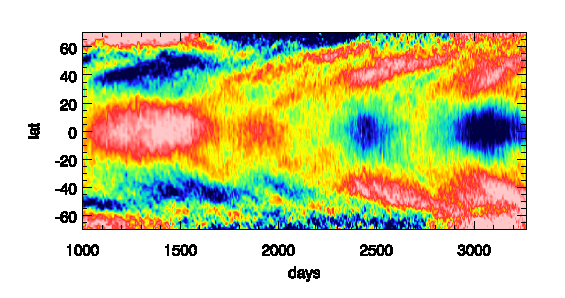
\includegraphics{figs/chapter_8/azav_mmc_vturf_3_SC2_12070_16700_Vp-avg-trace-0.85R_flucOmega.eps}
  \end{center}
  \caption[Time-dependent behavior in the cyclic case~D3b]
	  {Time-dependent behavior in the cyclic case~D3b.  $(a)$
	  Volume-averaged kinetic and magnetic energies, and 
	  $(b)$ mean $\langle B_\phi \rangle$ averaged over northern
	  and southern hemispheres at mid-convection zone.  Individual
          quantities are colored as in Fig.~\ref{fig:D3b}$a,b$.  Though
	  this simulation has evolved for only a short period, one
	  polarity reversal has already occurred.
	  $(c)$  Time-latitude maps of $\langle B_\phi \rangle$ at
	  mid-convection zone.  The large structures visible at the
	  poles near day 1500 appear to be part of the initial
	  transient as the dynamo equilibrates and adjusts the
	  profile of differential rotation.   
	  $(d)$   Time-latitude map of $\Omega'$ at mid-convection zone,
	  with time average removed to emphasize the poleward
	  propagating velocity structures. 
	  \label{fig:D3b}}
\end{figure*}

\begin{figure}
  \begin{center}
    \includegraphics{figs/chapter_8/mmc_vturf_3_SC2_patterns.eps}
%    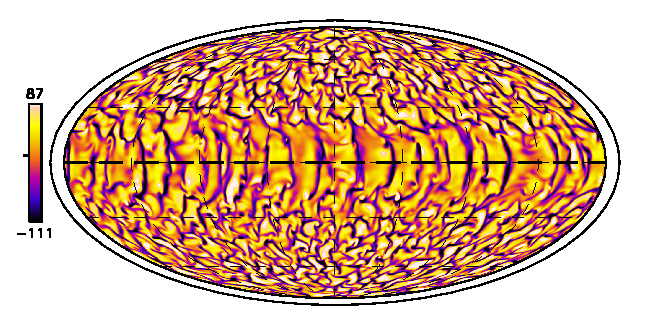
\includegraphics{figs/chapter_8/pub_mmc_vturf_3_SC2_shsl_14466_shell0_Vr.eps}
%    
\includegraphics{figs/chapter_8/pub_mmc_vturf_3_SC2_14466_14606_Vp.eps}\\
%    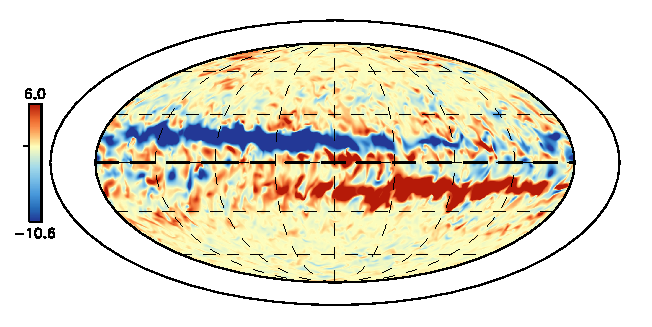
\includegraphics{figs/chapter_8/pub_mmc_vturf_3_SC2_shsl_14466_shell1_Bp.eps}
%    
\includegraphics{figs/chapter_8/pub_mmc_vturf_3_SC2_14466_14606_Bp.eps}\\
%    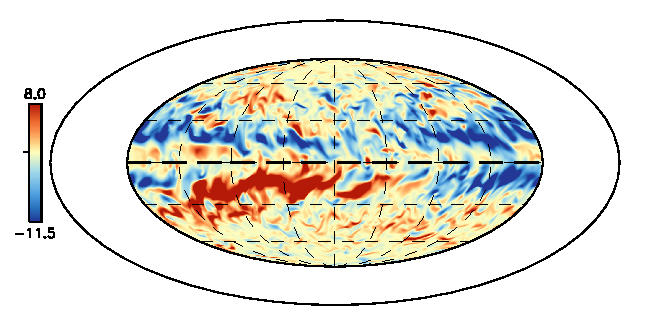
\includegraphics{figs/chapter_8/pub_mmc_vturf_3_SC2_shsl_14466_shell2_Bp.eps}
%    
\includegraphics{figs/chapter_8/pub_mmc_vturf_3_SC2_14466_14606_Bstream.eps}
  \end{center}
  \caption[Patterns of convection in case D3b]{Patterns of convection
  in case D3b.  $(a)$~Radial velocity $v_r$ in Mollweide projection
  near the top of the shell ($0.95\thinspace R_\odot$).  
  $(b)$~Toroidal magnetic field $B_\phi$ at mid-convection zone
  ($0.85\thinspace R_\odot$) with two wreaths of opposite polarity.  
  $(c)$~Wreaths near the bottom of the
  convective shell ($B_\phi$ at $0.73\thinspace R_\odot$).
  These snapshots are shown at day~2050, a time when the mean
  magnetic fields are strong.
  Also shown are 100 day averaged profiles of $(d)$~$\Omega$, 
  $(e)$~$\langle B_\phi \rangle$ and
  $(f)$~$\langle A_\phi \rangle$.
  \label{fig:D3b convection}} 
\end{figure}

The patterns of convection achieved in case~D3b are shown in
Figure~\ref{fig:D3b convection}.  The radial velocity structures are
more complex than in case~D3a and average amplitudes of
motion have increased a further 20\% (or roughly 35\% faster than the
radial flows in case~D3 at this depth).  The toroidal fields have 
amplitudes very similar to those realized in case~D3a, with typical
strengths of $\pm10$~kG at mid-convection zone and peak amplitudes of $\pm35$~kG.
The toroidal fields at the poles are much stronger in case~D3b than in
the previous $3\thinspace\Omega_\odot$ simulations, 
with fine-scale structure and typical field strengths of $\pm1.5$~kG.
In comparison, the polar $B_\phi$ of case~D3a had amplitudes of
$\pm1$~kG, while those fields in case~D3 rarely exceeded $\pm0.5$~kG
in amplitude.  The profiles of differential rotation
(Fig.~\ref{fig:D3b convection}$d$), mean toroidal magnetic field
(Fig.~\ref{fig:D3b convection}$e$) and the mean poloidal vector
potential (Fig.~\ref{fig:D3b convection}$f$) are all fairly similar to
those found in case~D3a.



\begin{figure*}[!t]
  \begin{center}
    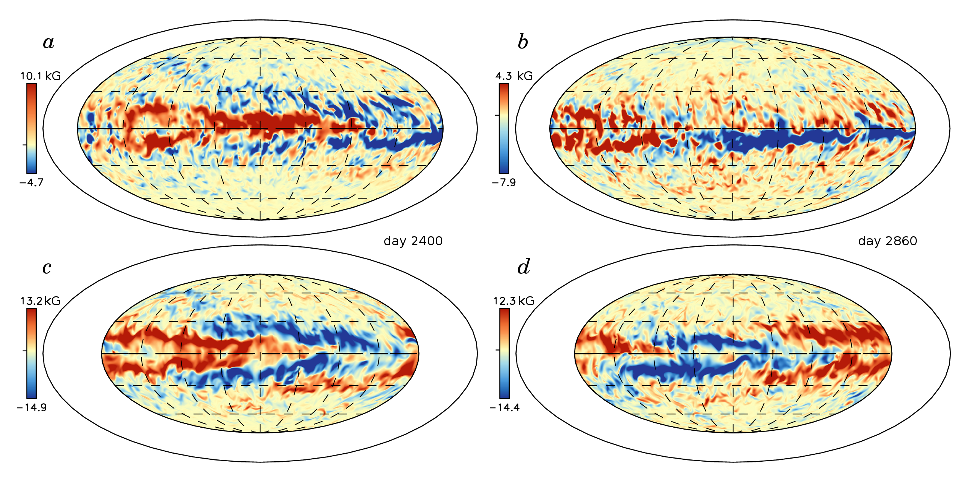
\includegraphics[width=\linewidth]{figs/chapter_8/case_D3b_patterns.eps}
  \end{center}
  \caption[$B_\phi$ achieving a more non-axisymmetric state in case~D3b]
	  {$B_\phi$ achieving a more non-axisymmetric state in case~D3b.    
  $(a)$~Mid-convection zone snapshot of
  $B_\phi$ at day~2400 and $(b)$~at day~2860.  At these times the
  wreaths have become highly non-axisymmetric structures.  
  $(c)$~Same fields near bottom of convection zone ($0.73\thinspace R_\odot$) at
  day~2400 and $(d)$~at day~2860.
  \label{fig:D3b two times}}
\end{figure*}

The wreaths of magnetism in case~D3b frequently attain strongly
non-axisymmetric states.  This is shown at two different times in
Figure~\ref{fig:D3b two times}.  At around day~2400 (Fig~\ref{fig:D3b
  two times}$a$), a region of reversed polarity appears in the midst of the southern
hemisphere.  This positive polarity $B_\phi$ replaces the preexisting
negative wreath, and is more equatorially located than the previous
wreaths (see Fig.~\ref{fig:D3b convection}$b$).  
The wreath in the northern hemisphere appears to peel apart and unwind
toward the north pole.  At this time the dynamo falls into a state
where the southern hemisphere is generating magnetic wreaths, while
the northern hemisphere is full of more complex structures, as near
day~2900 (Fig.~\ref{fig:D3b two times}$b$).  Here $\langle B_\phi
\rangle$ in the southern hemisphere is negative, but a positive
polarity structure of substantial amplitude occupies roughly 25\% of
the domain in longitude.  Near the bottom of the convection zone
(Fig.~\ref{fig:D3b two times}$c,d$) the story is similar.  There
are distinct wreath-like structures in each hemisphere, but individual
structures occupy only about $180^\circ$ in longitude before being
replaced by a structure with opposite polarity.  As a result of this
cancellation, $\langle B_\phi \rangle$ is very small in the lower convection zone.
In case~D3b the mean toroidal fields no longer dominate the structure
of the wreaths, and these structures must be analyzed on local scales. 



\section{High Pm Dynamos at $3~\Omega_\odot$}

To further probe the nature and sensitivity of these dynamo solutions we
explore a second path through parameter space where the magnetic
Prandtl number is increased.  Along this path, the viscous and thermal
diffusivities $\nu$ and $\eta$ are held constant while the magnetic
diffusivity $\eta$ is decreased, yielding larger magnetic Prandtl 
numbers and higher magnetic Reynolds numbers.  This path corresponds to
dynamo cases D3, D3-pm1, D3-pm2 and D3-pm4.  These dynamo simulations
begin occupying a similar region in parameter space as our previous
dynamo simulations conducted at the solar rotation rate
\citep[e.g.,][]{Brun_et_al_2004,Browning_et_al_2006}.  Along this
path, the magnetic Reynolds number increases while the fluid Reynolds
number should remain approximately constant, only changing as the
flows themselves respond to the magnetism that they generate.  
The convection retains a comparable level of complexity and the
underlying driving of the differential rotation should be nearly constant.

\begin{figure}
  \begin{center}
    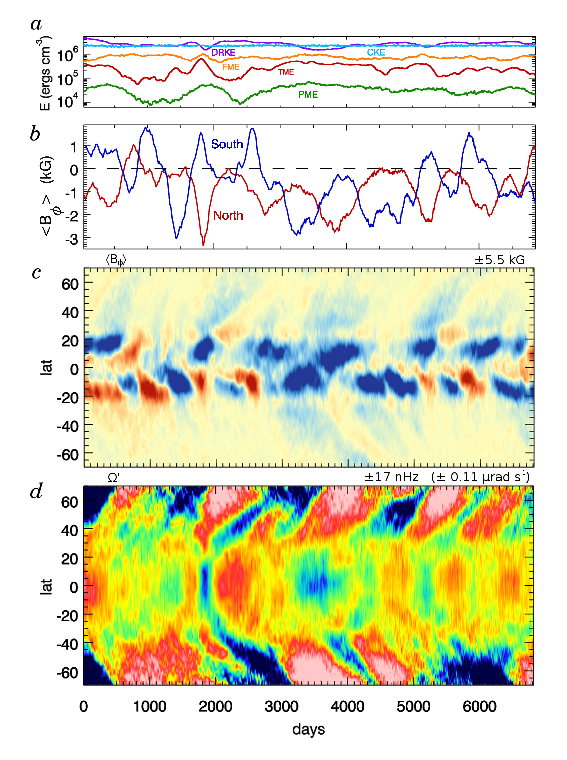
\includegraphics[width=0.8\linewidth]{figs/chapter_8/time_history_mmc_vturf_3_pm1.eps}
%    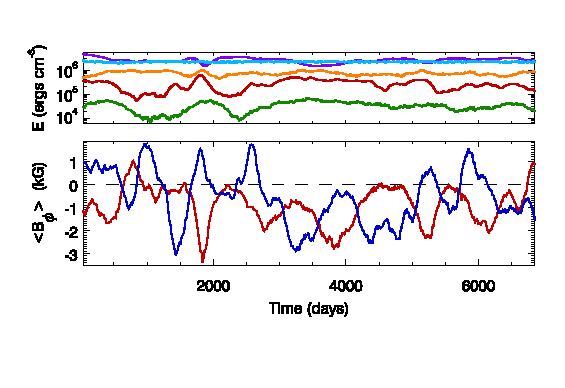
\includegraphics{figs/chapter_8/apj_dynamo_reversal_mmc_vturf_3_pm1_Bp-avg-trace-0.85R.eps}\\
%    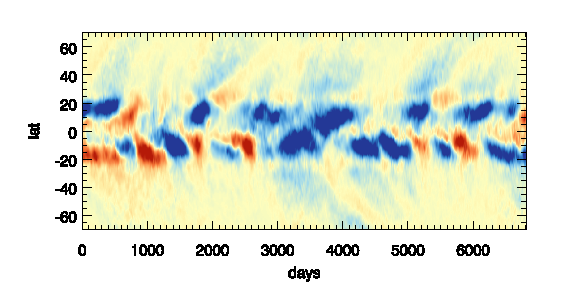
\includegraphics{figs/chapter_8/azav_mmc_vturf_3_pm1_4310_9990_Bp-avg-trace-0.85R.eps}\\
%    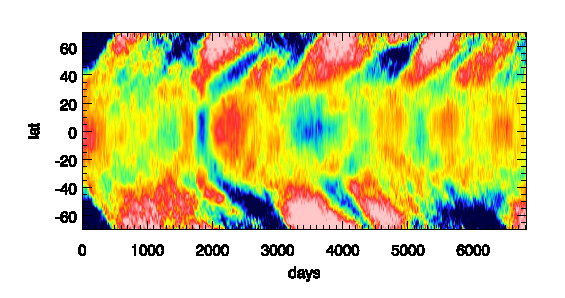
\includegraphics{figs/chapter_8/azav_mmc_vturf_3_pm1_4310_9990_Vp-avg-trace-0.85R_flucOmega.eps}
  \end{center}
    \caption[Time-dependent behavior in cyclic case~D3-pm1]
	  {Time-dependent behavior in cyclic case~D3-pm1.  $(a)$
	  Volume-averaged kinetic and magnetic energies, and 
	  $(b)$ mean $\langle B_\phi \rangle$ averaged over northern
	  and southern hemispheres at mid-convection zone.
	  $(c)$  Time-latitude maps of $\langle B_\phi \rangle$ at
	  mid-convection zone.    
	  $(d)$   Time-latitude map of $\Omega'$ at mid-convection zone,
	  with time average removed to emphasize the poleward
	  propagating velocity structures.
	  \label{fig:D3 pm1}}
\end{figure}

\textbf{Case~D3-pm1 --} At higher magnetic Prandtl numbers our dynamo
simulations also begin 
to experience significant time dependence.  This occurs already in our
first case, case~D3-pm1 with magnetic Prandtl number $\mathrm{Pm}=1$. 
The rms Reynolds number in this case is lower than in case~D3, with a
value of 149, owing to the weaker differential rotation realized in
this simulation.  The fluctuating Reynolds number is very similar with
a value of 102, but the rms and fluctuating magnetic Reynolds numbers
are higher than in that case, being 149 and 102 respectively. 

The time history of case~D3-pm1 is shown in Figure~\ref{fig:D3 pm1}.
At day~0 the values of $\eta$ in case~D3 were dropped by a factor of
two.  After about 500~days the steady wreaths from case~D3 begin to
break apart as new wreaths are generated near the equator.  This is
visible in time latitude maps of $\langle B_\phi \rangle$
(Fig.~\ref{fig:D3 pm1}$c$) at mid-convection zone.  The mean toroidal
fields hunt between states with two wreaths of opposite polarity and
states where one or two single polarity wreaths are built (i.e. days
3000-5000).  When two wreaths are present the simulation appears to
undergo frequent and rapid reversals, with typical timescales of only
a few hundred days.  Accompanying these reversals are strong angular
velocity structures that propagate toward the polar regions
(Fig.~\ref{fig:D3 pm1}$d$).

\begin{figure}
  \begin{center}
    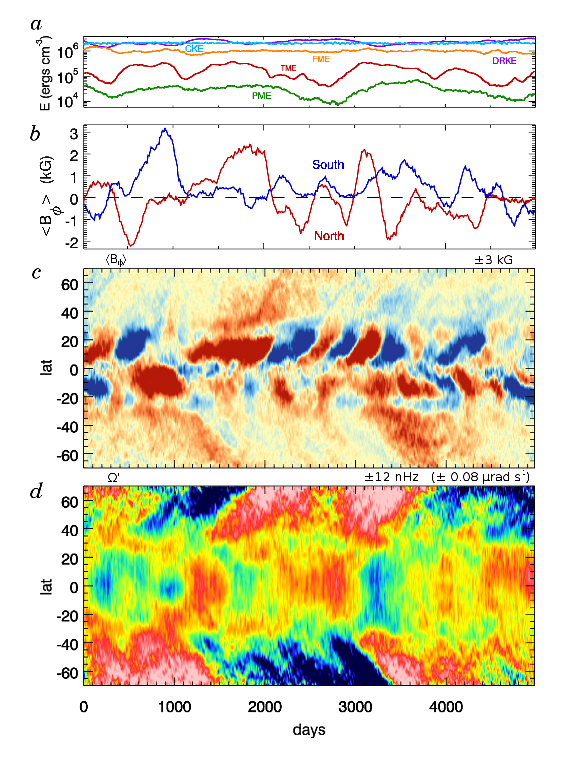
\includegraphics[width=0.8\linewidth]{figs/chapter_8/time_history_mmc_vturf_3_pm2.eps}
%    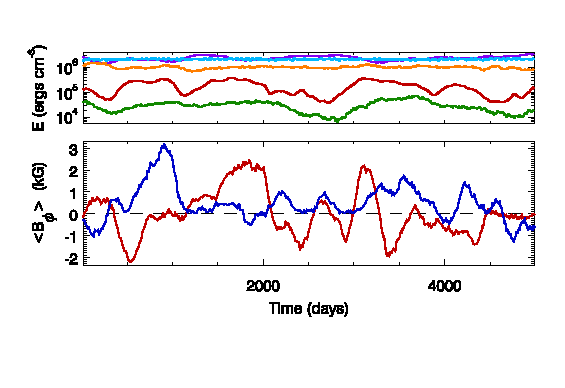
\includegraphics{figs/chapter_8/apj_dynamo_reversal_mmc_vturf_3_pm2_Bp-avg-trace-0.85R.eps}\\
%    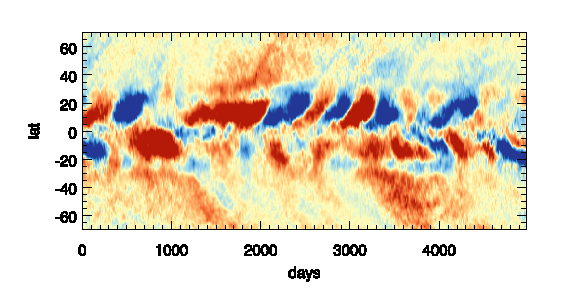
\includegraphics{figs/chapter_8/azav_mmc_vturf_3_pm2_4630_9430_Bp-avg-trace-0.85R.eps}\\
%    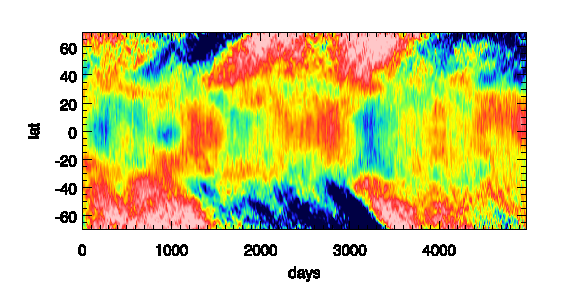
\includegraphics{figs/chapter_8/azav_mmc_vturf_3_pm2_4630_9430_Vp-avg-trace-0.85R_flucOmega.eps}
  \end{center}
    \caption[Time-dependent behavior in cyclic case~D3-pm2]
	  {Time-dependent behavior in cyclic case~D3-pm2.  $(a)$
	  Volume-averaged kinetic and magnetic energies, and 
	  $(b)$ mean $\langle B_\phi \rangle$ averaged over northern
	  and southern hemispheres at mid-convection zone.
	  $(c)$  Time-latitude maps of $\langle B_\phi \rangle$ at
	  mid-convection zone.  
	  $(d)$   Time-latitude map of $\Omega'$ at mid-convection zone,
	  with time average removed to emphasize the poleward
	  propagating velocity structures. 
	  \label{fig:D3 pm2}}
\end{figure}

\begin{figure}
  \begin{center}
    \includegraphics{figs/chapter_8/mmc_vturf_3_pm2_patterns.eps}
%    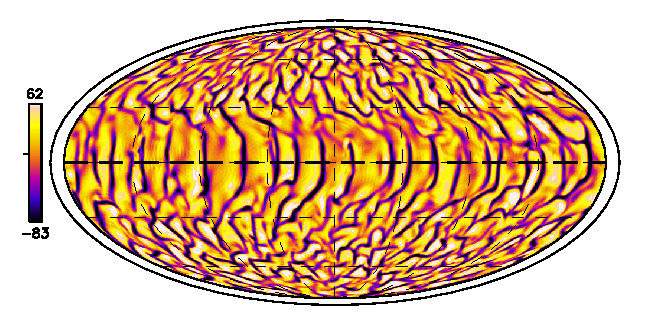
\includegraphics{figs/chapter_8/pub_mmc_vturf_3_pm2_shsl_7130_shell0_Vr.eps}
%    
\includegraphics{figs/chapter_8/pub_mmc_vturf_3_pm2_7100_7190_Vp.eps}\\
%    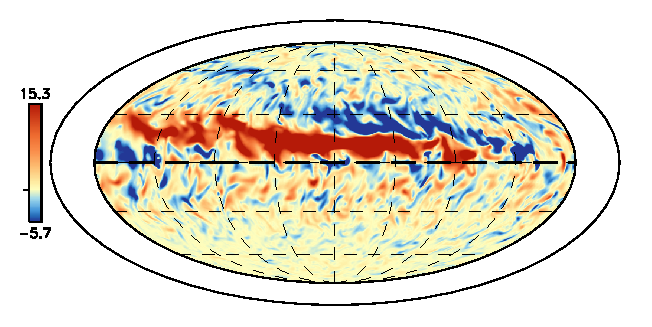
\includegraphics{figs/chapter_8/pub_mmc_vturf_3_pm2_shsl_7130_shell1_Bp.eps}
%    
\includegraphics{figs/chapter_8/pub_mmc_vturf_3_pm2_7100_7190_Bp.eps}\\
%    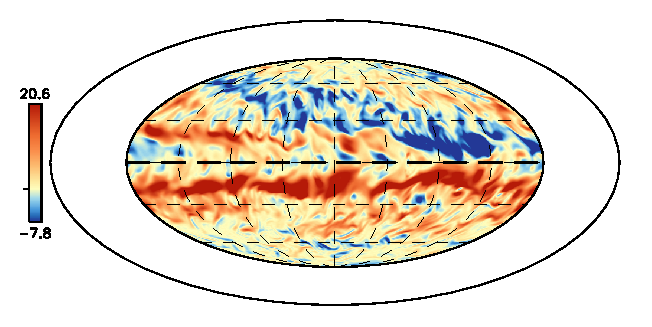
\includegraphics{figs/chapter_8/pub_mmc_vturf_3_pm2_shsl_7130_shell2_Bp.eps}
%    
\includegraphics{figs/chapter_8/pub_mmc_vturf_3_pm2_7100_7190_Bstream.eps}
  \end{center}
  \caption[Patterns of convection in case D3-pm2]
	  {Patterns of convection in case D3-pm2.  
  $(a)$~Radial velocity $v_r$ in Mollweide projection
  near the top of the shell ($0.95\thinspace R_\odot$).  
  $(b)$~Toroidal magnetic field $B_\phi$ at mid-convection zone
  ($0.85\thinspace R_\odot$) with one strong wreath.
  $(c)$~Two wreaths of same polarity are near the bottom of the
  convective shell ($B_\phi$ at $0.73\thinspace R_\odot$).
  These snapshots are shown at day~3100, a time when the mean
  magnetic fields are strong in the northern hemisphere.
  Also shown are 100 day averaged profiles of $(d)$~$\Omega$, 
  $(e)$~$\langle B_\phi \rangle$ and
  $(f)$~$\langle A_\phi \rangle$.
  \label{fig:D3 pm2 convection}} 
\end{figure}


\textbf{Case~D3-pm2 --} Our next case on the high magnetic Prandtl number path is case~D3-pm2,
with $\mathrm{Pm}=2$.  This case was initiated from case~D3-pm1, and
at roughly day 600 of that simulation the eddy diffusivity $\eta$ was
dropped by an additional factor of two, with $\nu$ and $\kappa$ still
the same as in case~D3.  
In this simulation the rms and fluctuating Reynolds numbers are almost
the same as in its progenitor (145 and 101 respectively), but the
magnetic Reynolds numbers have increase by a factor of two to values
of 291 and 202 for the rms and fluctuating quantities.

The time history for case~D3-pm2 is shown in
Figure~\ref{fig:D3 pm2}.  At first the wreaths
from the previous dynamo persist, but after about 250~days they are
replaced by different polarity structures and this dynamo diverges
strongly from its progenitor.  After about 1000 days the dynamo enters a
state where almost all $\langle B_\phi \rangle$ is located in the
northern hemisphere.  The dynamo undergoes cycles in that hemisphere
with the mean fields reversing on short timescales of a few hundred
days.  In the southern hemisphere the mean fields are weaker but are
able to retain their average polarity and do not experience as many
reversals.  Angular velocity features launch toward the north pole
frequently.  These structures occasionally occur in the southern
hemisphere, when the mean magnetic fields become particularly strong
(i.e. days 3000-3800).




The patterns of convection in case~D3-pm2 are shown in
Figure~\ref{fig:D3 pm2 convection}.  Near the surface, the convective
cells are very similar to those found in our other simulations at
three times the solar rate with velocities similar to those in
case~D3, rather than the faster flows found in cases~D3a and D3b.  The
magnetic fields in this case are much stronger and show marked
asymmetry, with strong fields occupying narrow ranges of longitude.
At mid-convection zone, often a single strong wreath appears in the
northern hemisphere.  These states are similar to those realized
occasionally in case~D5, and as there, weaker opposite polarity field
surrounds the single wreath.  At greater depths, two wreaths of the
same polarity occupy the two hemispheres.
A profile of the mean differential rotation (angular velocity $\Omega$) 
is shown averaged over a 100 day interval around the snapshots
(Fig.~\ref{fig:D3 pm2 convection}$d$).  Accompanying profiles show
$\langle B_\phi \rangle$ and $\langle A_\phi \rangle$ averaged over the
same interval (Fig.~\ref{fig:D3 pm2 convection}$e,f$).  During this
interval, the wreaths possess a substantially different mean poloidal
field than in our previous simulations at three times the solar rate.
Here the mean poloidal field is almost quadrupolar in nature.



\textbf{Case~D3-pm4 --}
Our highest magnetic Prandtl number case at three times the solar
rate is case~D3-pm4 with $\mathrm{Pm}=4$.  This simulation is quite
magnetically turbulent.  The rms and fluctuating Reynolds numbers remain comparable
to the other simulations on the high-$\mathrm{Pm}$ branch, with values
of 161 and 94 respectively.  The magnetic
Reynolds numbers are much higher, with rms and fluctuating values of
644 and 377.  The fluctuating magnetic Reynolds number is among the
highest achieved in any of our rapidly rotating dynamo simulations and
is comparable to those achieved in previous simulations of the solar
dynamo \citep{Brun_et_al_2004, Browning_et_al_2006}.  Despite this
high level of magnetic turbulence, case~D3-pm4 still builds significant
magnetic wreaths within its convection zone.  
% NOTE to self: Make sure that the new values of D3-pm4 are put in as
% this thing equilibrates over the next month.  BPB 7/29/09 \textbf{} 


\clearpage

\begin{figure}[!p]
  \begin{center}
%    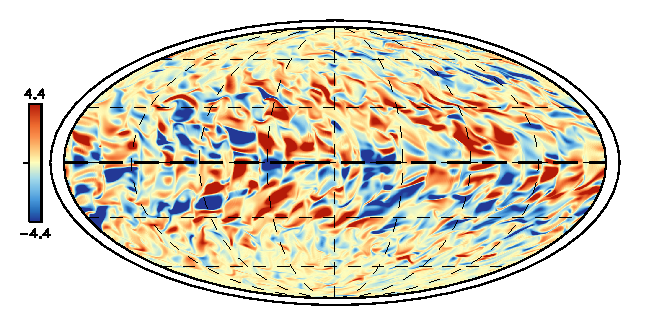
\includegraphics{figs/chapter_8/pub_mmc_vturf_3_pm4_shsl_4510_shell0_Bp.eps}\\
    \includegraphics{figs/chapter_8/mmc_vturf_3_pm4_patterns.eps}
%    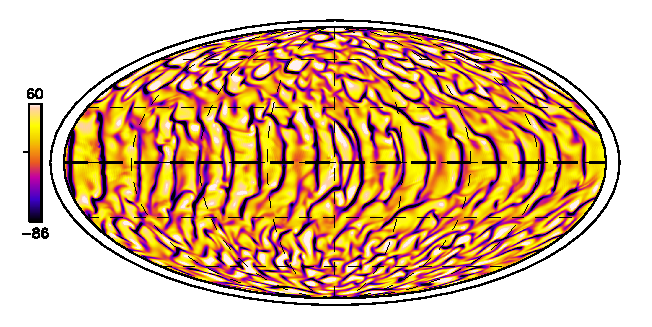
\includegraphics{figs/chapter_8/pub_mmc_vturf_3_pm4_shsl_4510_shell0_Vr.eps}\\
%    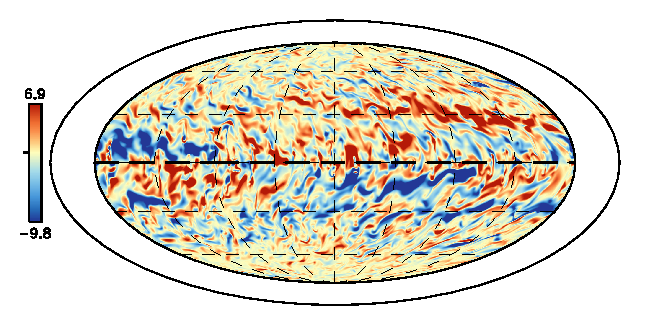
\includegraphics{figs/chapter_8/pub_mmc_vturf_3_pm4_shsl_4510_shell1_Bp.eps}\\
%    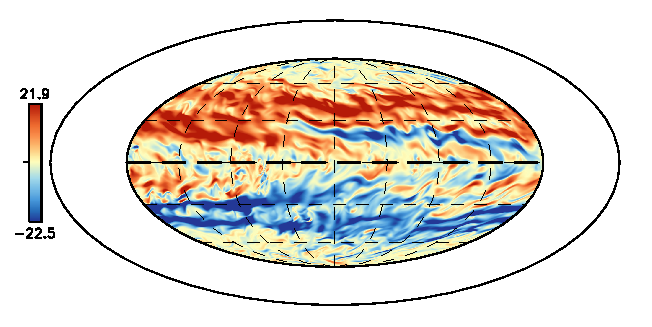
\includegraphics{figs/chapter_8/pub_mmc_vturf_3_pm4_shsl_4510_shell2_Bp.eps}
  \end{center}
  \caption[Patterns of convection in case D3-pm4]
	  {Patterns of convection in case D3-pm4.  
  $(a)$~Radial velocity $v_r$ in Mollweide projection
  near the top of the shell ($0.95\thinspace R_\odot$).  
  $(b)$~Toroidal magnetic field $B_\phi$ at mid-convection zone
  ($0.85\thinspace R_\odot$) with indistinct wreaths.
  $(c)$~Two strong wreaths are at high latitudes near the bottom of the
  convective shell ($B_\phi$ at $0.73\thinspace R_\odot$).
  These snapshots are shown at day~1830.  The dynamo is still
  equilibrating at this time.
  Also shown are 20 day averaged profiles of $(d)$~$\Omega$, 
  $(e)$~$\langle B_\phi \rangle$ and
  $(f)$~$\langle A_\phi \rangle$.
  \label{fig:D3 pm4 convection}}
\end{figure}




The patterns of convection and the magnetic
structures realized are shown in Figure~\ref{fig:D3 pm4 convection} at
a time shortly after the dynamo has equilibrated.  Though the velocity
patterns remain very similar, the magnetic fields have significantly
more fine-scale structure.
Though highly complex at mid-convection zone, the toroidal fields
retain an overall polarity in each hemisphere
(Fig.~\ref{fig:D3 pm4 convection}$b$).  Near the bottom of the
convection zone the wreaths again are marked by the strong mean
fields (Fig.~\ref{fig:D3 pm4 convection}$c,e$).  Indeed, the magnetic
fields generated within these wreaths are among the strongest
achieved in any of our rapidly rotating dynamos, with typical
amplitudes of more than $\pm20\:$kG in the fluctuating fields and peak
amplitudes of $\pm40\:$kG near the base of the convection zone.  This simulation has
only experienced about 1800 days of evolution and the timesteps are
heavily limited by the Alfv\'enic CFL with typical limits near 30
seconds or less.


\section{Resulting Differential Rotation}
In our high magnetic Prandtl number branch of simulations, we find that the
mean profile of differential rotation is somewhat different than in
our $\mathrm{Pm}=0.5$ simulations. In these higher magnetic Prandtl
number cases, the equator remains prograde with more retrograde poles,
but the overall angular velocity contrast is significantly weaker.
Measurements of the angular velocity contrast in latitude and in
radius are shown for all of our dynamos at three times the solar rate
in Table~\ref{table:delta_omega_D3_branch}.  These values are
time-averaged over the indicated ranges of dates and these intervals
typically span several magnetic oscillations or reversals.
Case~D3b is still undergoing some
evolution in $\Delta \Omega$ at this time, as is case~D3-pm4, which
has seen approximately 1800~days of evolution and has uncertain
time-dependence. The other cases are well equilibrated.
Accompanying each measurement is an indication of the standard
deviation of the angular velocity contrast in time, with case~D3
showing little variation and the more turbulent cases showing
substantially larger excursions.  

\clearpage 

\begin{deluxetable}{lcccc}
    \tabletypesize{\footnotesize}
    \tablecolumns{5}
    \tablewidth{0pt}  % `natural' size 
    \tablecaption{Mean $\Delta \Omega$ in Dynamos at $3\thinspace\Omega_\odot$
    \label{table:delta_omega_D3_branch}}
    \tablehead{\colhead{Case}  &  
      \multicolumn{2}{c}{$\Delta \Omega_{\mathrm{lat}}$} &
      \colhead{$\Delta \Omega_\mathrm{r}$} &
      \colhead{Epoch} \\
      \colhead{} &
      \colhead{$0.97 R_\odot$} &
      \colhead{$0.85 R_\odot$} &
      \colhead{equator} &
      \colhead{days}
   }
   \startdata
    D3     &   1.18 $\pm$ 0.05 &   0.79 $\pm$ 0.06 &   0.70 $\pm$ 0.02 &   $2000\phn -  \phn6980$ \\
    D3a    &   1.11 $\pm$ 0.18 &   0.68 $\pm$ 0.10 &   0.71 $\pm$ 0.13 &   $2000\phn - 15980$ \\
    D3b    &   1.01 $\pm$ 0.17 &   0.56 $\pm$ 0.07 &   0.71 $\pm$ 0.14 &   $1000\phn -  \phn3120$ \\[3mm]
    %
    D3-pm1 &   0.87 $\pm$ 0.10 &   0.53 $\pm$ 0.07 &   0.55 $\pm$ 0.06 &   $1000\phn -  \phn6850$ \\
    D3-pm2 &   0.78 $\pm$ 0.08 &   0.48 $\pm$ 0.05 &   0.48 $\pm$ 0.06 &   $1000\phn -  \phn4730$ \\
    D3-pm4 &   0.90 $\pm$ \phn\phn ?\phn   &   0.74 $\pm$ \phn\phn ?\phn    &   0.38 $\pm$ \phn\phn ?\phn    &   $1830\phn -  \phn1850$                    
    % These measurements performed 4/1/2009; see worklog for details
    \enddata
    \vskip-0.5cm
    \tablecomments{Angular velocity shear in units of $\mu
    \mathrm{rad}\: s^{-1}$, with $\Delta \Omega_\mathrm{lat}$ measured
    at two depths and $\Delta \Omega_\mathrm{r}$ measured across the
    full shell at the equator.  %Also indicated are standard deviations
%   in time of these differences. These measurements are averaged over
%   the indicated range of days.  Case~D3b is still undergoing
%   some evolution in $\Delta \Omega$ at this time, as is
%   case~D3-pm4, which has seen approximately 1800~days of evolution
%   and has uncertain time-dependence.
%   The other cases are well equilibrated
}
\end{deluxetable}



In the $\mathrm{Pm}=0.5$ branch of dynamos, the more turbulent dynamos
still have a strong differential rotation.  The latitudinal angular
velocity contrast $\Delta \Omega_\mathrm{lat}$ in the upper convection
zone decreases slightly as the diffusivities are dropped.  At
mid-convection zone the decrease is stronger.  In contrast, the
radial shear at the equator remains almost constant in this group of
cases.  
The high magnetic Prandtl number dynamos have differential rotation
profiles that become substantially weaker as $\eta$ is decreased.  In
this family of solutions, both the latitudinal and radial shear are
markedly smaller.  In comparing to the $\mathrm{Pm}=0.5$ dynamos,
case~D3-pm1 and case~D3b, with similar values of $\eta$ throughout the
convection zone, have similar latitudinal shear at mid-convection zone
but different angular velocity contrasts in the upper convection zone
and in radius.



\section{Extreme Rotators: $10$ and $15~\Omega_\odot$ dynamos}

Our most rapidly rotating dynamo simulations are currently at ten and
fifteen times the current solar rotation rate.  In a star like our
Sun, such rapid rotation is likely only when the star is very young,
shortly after reaching the main sequence.  In these stars, we find that
the dynamos can produce magnetic fields which are strong enough to
largely quench the differential rotation.  Despite this, cyclic
oscillations and global-scale polarity reversals of the mean magnetic
fields continue to occur.  

In total, there are three simulations rotating in this regime.  Two of
these simulations are rotating at $10~\Omega_\odot$, one with the same
diffusivities used in case~D5 (case~D10L) and one with lower
diffusivities in keeping with the scaling law of
equation~\ref{eq:diffusivity scaling} (case~D10).  Our most rapidly
rotating dynamo is case~D15, at $15~\Omega_\odot$.  Here we will
briefly examine the emergence of nests of convection in case D10L, and
the suppression of differential rotation in case~D15.


\textbf{Case~D10L --} 
Only one of our most rapidly rotating cases retains a strong
differential rotation.  This is case~D10L rotating at
$10\thinspace\Omega_\odot$ and with eddy diffusivities identical to
those in both case~D5 and case~D3a.  Typical rms and fluctuating
Reynolds numbers in this simulation are 331 and 110 respectively, with
rms and fluctuating magnetic Reynolds numbers of 165 and 55.  The time
history of case~D10L is shown in Figure~\ref{fig:D10L}, covering
6000~days of the simulation after the initial seed magnetic fields are
introduced.  The magnetic energies grow quickly to near equipartition
with the kinetic energies before they react back on the differential
rotation and substantially suppress~it.  

\begin{figure*}
  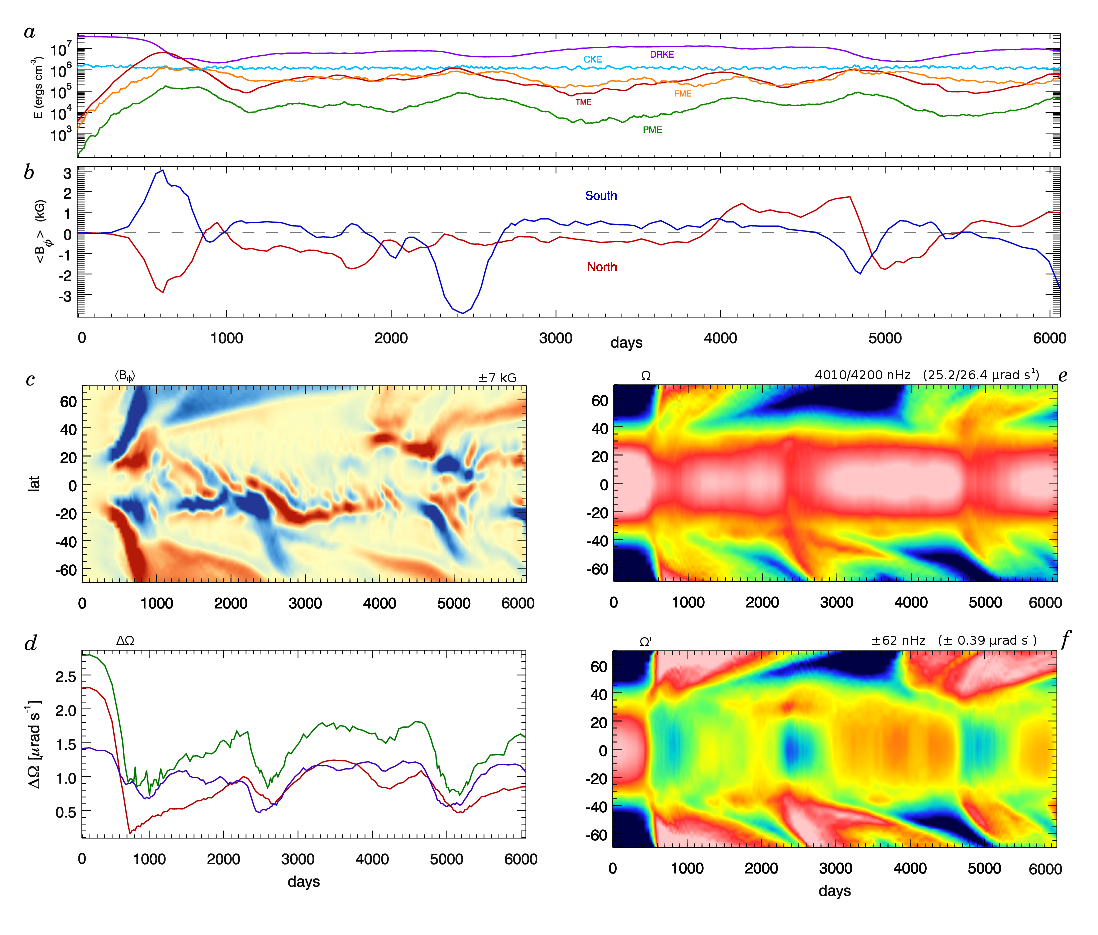
\includegraphics[width=\linewidth]{figs/chapter_8/time_history_mmc_vturf_10_LC.eps}
%  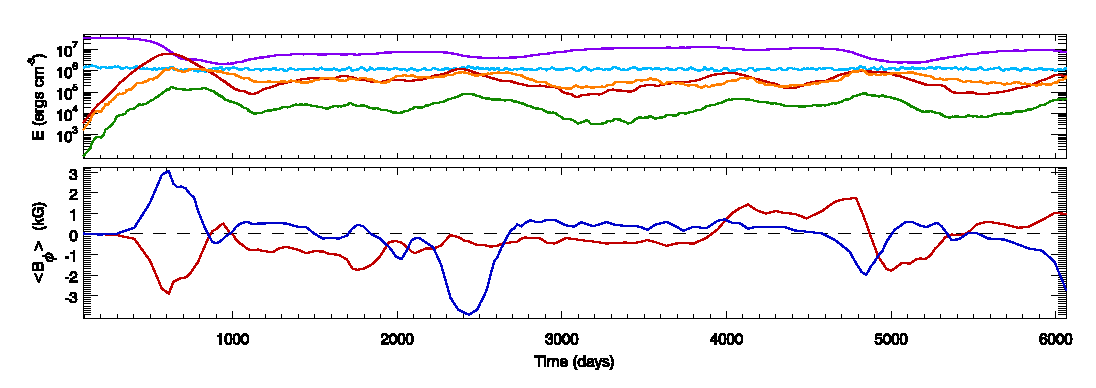
\includegraphics[width=\linewidth]{figs/chapter_8/mmc_vturf_10_LC/apj_dynamo_reversal_mmc_vturf_10_LC_Bp-avg-trace-0.85R.eps}\\
%  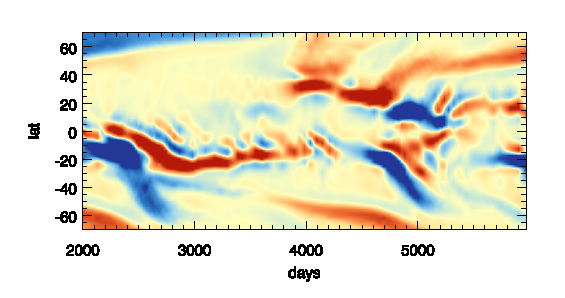
\includegraphics[width=0.5\linewidth]{figs/chapter_8/mmc_vturf_10_LC/azav_mmc_vturf_10_LC_5210_6680_Bp-avg-trace-0.85R.eps}
%  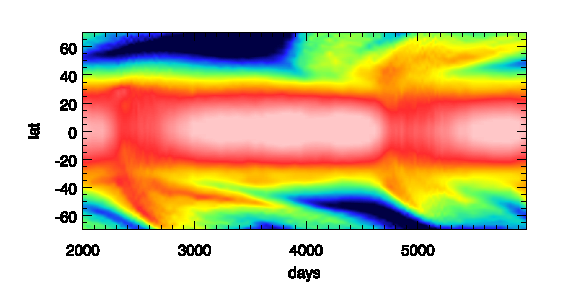
\includegraphics[width=0.5\linewidth]{figs/chapter_8/mmc_vturf_10_LC/azav_mmc_vturf_10_LC_5210_6680_Vp-avg-trace-0.85R_Omega.eps}\\
%  \includegraphics[width=0.5\linewidth]{figs/chapter_8/mmc_vturf_10_LC/delta_omega_azav_mmc_vturf_10_LC_5210_6680_Vp-avg-trace-0.97R.eps}
%  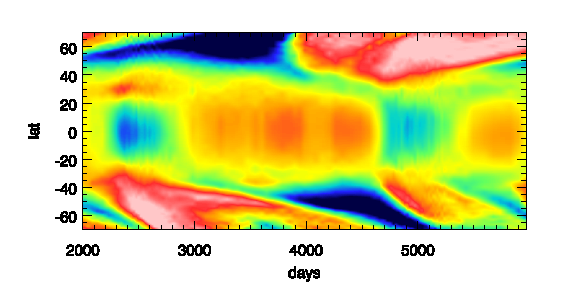
\includegraphics[width=0.5\linewidth]{figs/chapter_8/mmc_vturf_10_LC/azav_mmc_vturf_10_LC_5210_6680_Vp-avg-trace-0.85R_flucOmega.eps}\\
  \caption[Time-dependent behavior in case~D10L]
	  {Time-dependent behavior in case~D10L.  
          $(a)$~Volume-averaged kinetic and magnetic energies, and 
	  $(b)$~mean $\langle B_\phi \rangle$ averaged over northern
	  and southern hemispheres at mid-convection zone.
	  $(c)$~Time-latitude maps of $\langle B_\phi \rangle$ at
	  mid-convection zone.
          $(d)$~Angular velocity contrast $\Delta \Omega$, with
          $\Delta \Omega_\mathrm{lat}$ measured near the surface (top
          line, green) and at mid-convection zone (bottom line, red)
          and with $\Delta \Omega_r$ measured across the shell at the
          equator (middle line, purple). 
	  $(e)$~Time-latitude map of full angular velocity $\Omega$ at
          mid-convection zone, with fast equator and slow poles.
	  $(f)$~Map of $\Omega'$ with time average removed,
          emphasizing temporal variations.  The initial transient
          slows the equator and speeds up the poles, reducing the
          overall differential rotation.
          \label{fig:D10L}}
\end{figure*}


    Time-latitude maps of $\langle B_\phi \rangle$ and $\Omega$
reveal how this quenching occurs. 
Case~D10L builds strong wreaths of magnetism which frequently
propagate toward the polar regions (Fig.~\ref{fig:D10L}$c$).  
These poleward-slips of
$\langle B_\phi \rangle$ are accompanied by substantial poleward
propagating angular velocity structures, which transport quickly
rotating material from the prograde equator to the retrograde poles.
This is evident in the time-evolution of the latitudinal and radial
angular velocity contrast $\Delta \Omega$ (Fig.~\ref{fig:D10L}$d$).
During the initial transient, the latitudinal angular velocity
contrast  $\Delta \Omega_\mathrm{lat}$ is substantially reduced,
dropping by a factor of about two in the upper convection zone and by
nearly a factor of five at mid-convection zone.  Convection rebuilds
the differential rotation and by day~2300 nearly half the angular
velocity contrast has been rebuilt.  At this point however, strong
magnetic wreaths are formed leading to another pulse of poleward
propagating fields and flows.  The radial angular velocity contrast
$\Delta \Omega_r$ is less affected by the magnetism.  It experiences
temporal variations on similar timescales, but retains an average
value similar to the hydrodynamic progenitor (visible at day~0).

\begin{figure*}[!t]
  \begin{center}
    \includegraphics{figs/chapter_8/mmc_vturf_10_LC_mean_flows.eps}
%    \includegraphics{figs/chapter_8/mmc_vturf_10_LC/pub_mmc_vturf_10_LC_6280_6289_Vp.eps}
%    \includegraphics{figs/chapter_8/mmc_vturf_10_LC/pub_mmc_vturf_10_LC_6280_6289_Bp.eps}
%    \includegraphics{figs/chapter_8/mmc_vturf_10_LC/pub_mmc_vturf_10_LC_6280_6289_Bstream.eps}
  \end{center}
  \caption[Differential rotation and magnetism in case~D10L]
          {Differential rotation and magnetism in case~D10L.
          $(a)$~Profile of angular velocity $\Omega$ averaged over an
          interval of about 100 days when the differential rotation is
          strong (days 4490-4600) accompanied by $(b)$~radial
          cuts.  $(c)$~Two magnetic wreaths are present.  
          $(d)$~The~poloidal vector potential $\langle A_\phi \rangle$
          is complex and largely of a single polarity.
          \label{fig:D10L mean flows}}
\end{figure*}

The mean toroidal magnetic fields have a much more complex structure
than in our three or five solar dynamos.  Strong concentrations of $\langle
B_\phi \rangle$ appear and disappear on short timescales near the
equator while large wreaths occupy latitudes near $\pm 20^\circ$.
Those wreaths eventually slip toward the poles and are often replaced
by wreaths of opposite polarity (i.e. the reversals that occur near
day~2500 and day~4900).  Though initially the dynamo builds quite
symmetric wreaths, the wreaths which form after the initial transient
are less symmetric and frequently are substantially stronger in one
hemisphere and weaker in the other.

Time-averaged profiles in radius and latitude of the differential
rotation and the magnetic fields are shown in Figure~\ref{fig:D10L
mean flows} at a time when the differential rotation is strong
(days~4490-4600).  The equatorial regions still possess a strong radial
shear, and the profile and radial cuts are similar to cases~D3 and
D5.  Two magnetic wreaths are formed, with a strong positive polarity
in the northern hemisphere and a weaker wreath in the southern.  Here
the poloidal field is quite complex and is highly asymmetric with
a major enhancement of $\langle A_\phi \rangle$ visible in the
northern hemisphere.  This is in marked contrast to the poloidal
fields achieved in our cases at three times the solar rate, which were
dominated by low-$\ell$ structures with typically either
largely octopolar (i.e. cases~D3, D3$a$, D3$b$) or quadrupolar
(i.e. case~D3-pm2) topologies. 


%\begin{sidewaysfigure}
\begin{figure}[!t]
  \includegraphics[width=\linewidth]{figs/chapter_8/D10_L_patch.eps}
  \caption[Convective patterns in case~D10L with nests of convection]
          {Convective patterns in case~D10L with nests of convection.
            Shown as snapshots in Mollweide projection are radial
            velocities $v_r$ $(a)$~near the surface ($0.95\thinspace
            R_\odot$) and $(b)$~at mid-convection zone
            ($0.85\thinspace R_\odot$).  Two active nests of
            convection are clearly visible.  $(c)$~Near the surface,
            the radial magnetic field $B_r$ is concentrated in the
            stronger nest.  $(d)$~At mid-convection zone the active
            nests make an imprint on the magnetic wreaths. 
            Also visible near the south pole are the 
            remnants of the magnetic wreath from the previous cycle.
            These snapshots are of day~4490 at a period when the
            differential rotation is strong. 
            \label{fig:D10L convection}}
\end{figure}
%\end{sidewaysfigure}

The patterns of convection in case~D10L are unique among our rapidly
rotating dynamos.  The relatively strong differential rotation,
combined with the rapid overall rotation, lead to strongly localized
nests of convection in the equatorial regions.  These
nests are shown in Figure~\ref{fig:D10L convection} at day~4490, when
the differential rotation is strong.  The localized convection once
again is strongly visible in the radial velocity patterns throughout
the convection zone (Fig.~\ref{fig:D10L convection}$a,b$).  At this
instant, two nests are visible, separated by almost $180^\circ$ of
longitude.  

The nests have substantial magnetic signatures as well,
particularly in the radial magnetic field near the surface
(Fig.~\ref{fig:D10L convection}$c$).  Here the stronger nest (at left)
is accompanied by a significant enhancement of radial field.  At
mid-convection zone the nests also make an imprint on the toroidal
field, locally stretching and shredding the wreaths.  In the more
quiescent regions between the nests, the wreaths are stronger and
have less fine-scale structure (Fig.~\ref{fig:D10L convection}$d$).

In case~D10L the active nests of convection are clearly visible and
persist for many hundreds of days.  The temporal variations in the
differential rotation lead to periods when the nests are strong and
the convection is highly confined in longitude, as well as other
periods where the differential rotation and nests are weaker.
Time-longitude maps reveal that on thousand day timescales the convection
alternates between states with two or three active nests, spending a
few hundred days in each state.



\textbf{Cases~D10 --} Our other dynamo at ten times the solar rate is
case~D10, with diffusivities lower by slightly more than a factor of
two compared to case~D10L.  This simulation is more turbulent, with
rms and fluctuating Reynolds numbers of 253 and 228 and rms and
fluctuating magnetic Reynolds numbers of 126 and 114 respectively.
The small spread between the rms and fluctuating values is due to the
differential rotation collapsing almost entirely.

\begin{deluxetable}{lcccc}
    \tabletypesize{\footnotesize}
    \tablecolumns{5}
    \tablewidth{0pt}  % `natural' size 
    \tablecaption{Mean $\Delta \Omega$ in Dynamos at $10$ and $15\thinspace\Omega_\odot$
    \label{table:delta_omega_fast_dynamos}}
    \tablehead{\colhead{Case}  &  
      \multicolumn{2}{c}{$\Delta \Omega_{\mathrm{lat}}$} &
      \colhead{$\Delta \Omega_\mathrm{r}$} &
      \colhead{Epoch} \\
      \colhead{} &
      \colhead{$0.97 R_\odot$} &
      \colhead{$0.85 R_\odot$} &
      \colhead{equator} &
      \colhead{days}
   }
   \startdata
   D10L  &   1.39 $\pm$ 0.27 &   0.83 $\pm$ 0.21 &   0.97 $\pm$ 0.19 &   $1000-  6060$ \\
   D10   &   0.45 $\pm$ 0.08 &   0.22 $\pm$ 0.05 &   0.38 $\pm$ 0.10 &   $2720-  5000$ \\[3mm] 
   %
   D15   &   0.33 $\pm$ 0.07 &   0.12 $\pm$ 0.04 &   0.26 $\pm$ 0.08 &   $1500-  4500$ \\
   D15   &   0.30 $\pm$ 0.04 &   0.10 $\pm$ 0.01 &   0.22 $\pm$ 0.03 &   $2000-  3500$ \\
   D15   &   0.51 $\pm$ 0.01 &   \phn0.17 $\pm$ 0.003 &  0.50 $\pm$ 0.02 &   $3950-  4100$
    % These measurements performed 4/1/2009; see worklog for details
    \enddata
    \vskip-0.5cm
    \tablecomments{Angular velocity shear in units of $\mu
   \mathrm{rad}\: s^{-1}$, with $\Delta \Omega_\mathrm{lat}$ measured
   at two depths and $\Delta \Omega_\mathrm{r}$ measured across the
   full shell at the equator.  These measurements are averaged over
   the indicated range of days.  Dynamo case D15 suddenly amplifies
   its differential rotation for a period of time between days
   3700-4300.}
\end{deluxetable}

The average angular velocity contrast achieved in these most rapidly
rotating simulations is reported in
Table~\ref{table:delta_omega_fast_dynamos}.  In case~D10, the angular
velocity contrast $\Delta \Omega$ and its temporal variations have
both become much smaller than 
in case~D10L.  These quantities are measure over an interval of almost
2300~days.  There is little angular velocity contrast in either radius
or latitude.  

Despite the small differential rotation, substantial toroidal magnetic
fields are generated throughout the convection zone.  Now however, the
mean fields comprise a smaller proportion of the total magnetic energy
while the fluctuating fields become more prominent.  The fluctuations
exist on large scales, and with substantial contributions from
longitudinal wavenumbers m=1 or m=2.  The structure of the
magnetic fields remains wreath-like, though now more complex.  The
wreaths appear to still undergo cyclic variations in polarity.


\textbf{Case~D15 --} In our most rapidly rotating dynamo, case~D15,
the differential rotation is even weaker.  This dynamo is one of the
more turbulent $\mathrm{Pm}=0.5$ dynamos, with a fluctuating
Reynolds number of 272 and a fluctuating magnetic Reynolds number of
136.  This case is thus comparable to case~D3b.  The hydrodynamic
progenitor to this case had a very strong differential rotation, and
its rms and fluctuating Reynolds numbers were 1670 and 293 respectively.


\begin{figure*}
  \includegraphics[width=\linewidth]{figs/chapter_8/time_history_mmc_vturf_15.eps}
  \caption[Time-dependent behavior in case~D15]
	  {Time-dependent behavior in case~D15.  
          $(a)$~Volume-averaged kinetic and magnetic energies, and
            $(b)$~mean $\langle B_\phi \rangle$ averaged over northern
            and southern hemispheres at mid-convection zone.  The
            azimuthally averaged data exists from day~660 onwards.
            $(c)$~Time-latitude maps of $\langle B_\phi \rangle$ at
            mid-convection zone.  $(d)$~Angular velocity contrast
            $\Delta \Omega$, with $\Delta \Omega_\mathrm{lat}$
            measured near the surface (top line, green) and at
            mid-convection zone (bottom line, red) and with $\Delta
            \Omega_r$ measured across the shell at the equator (middle
            line, purple).  The latitudinal differential rotation is
            highly suppressed after the dynamo equilibrates, but the
            radial shear at the equator is largely unaffected.
            $(e)$~Time-latitude map of full angular velocity $\Omega$
            at mid-convection zone.  $(f)$~Map of $\Omega'$ with
            time-average removed, emphasizing temporal variations.
            The initial transient slows the equator and speeds up the
            poles, reducing the overall differential rotation.  In
            this dynamo, the poles actually become prograde, and
            retain that sense for long intervals.
          \label{fig:D15}}
\end{figure*}

The time history of case~D15 is shown in Figure~\ref{fig:D15}.
Starting from weak seed fields, the dynamo quickly builds strong
magnetic wreaths whose energies on average reach equipartition with
the convective flows.  These fields quench the differential rotation,
driving DRKE down into sub-equipartition with either the convection
(CKE) or the fluctuating magnetism.
Though the differential rotation is weak, the dynamo still undergoes
substantial temporal variations and cycles of polarity change
(Fig.~\ref{fig:D15}$b$).  Time-latitude maps reveal that, as in
case~D3-pm2, this cyclic wreath building activity is largely confined
to the northern hemisphere (Fig.~\ref{fig:D15}$c$).  The wreaths that
are achieved begin to slip toward the north pole almost immediately,
and typically persist in the equatorial region for less than 500~days
before beginning their poleward migration.

\clearpage
The first magnetic wreaths that form were two strong wreaths of opposite
polarity in the two hemispheres.  These first magnetic wreaths slip to the poles
and transport enough angular momentum from the prograde equator that
above $\pm 70^\circ$ the polar regions change their sense of
differential rotation from retrograde to prograde.  Once prograde
flows are established in the polar regions, they persist for the full
5000 simulated days shown here.  The angular velocity contrasts become
much weaker after the dynamo saturates and reduces the differential
rotation.  As in case~D10L, the latitudinal contrast is affected
more strongly by the magnetism than the radial shear, though $\Delta \Omega_r$
also decreases significantly (Fig.~\ref{fig:D15}$d$).  Dynamo case~D15 has
latitudinal and radial angular velocity contrasts which range from  
$0.3$ to $0.5\thinspace\mu \mathrm{rad}\: s^{-1}$ depending on the phase
of the dynamo oscillations (see Table~\ref{table:delta_omega_fast_dynamos}). 
During a brief period (days 3800\medspace-\thinspace4500) the differential rotation in
the upper convection zone becomes substantially stronger, with both
the latitudinal and radial shear increasing by more than a factor of
two.  The mid-convection zone $\Delta \Omega$ shows almost no
variation during this interval. 
Even at their peak levels (about day 400), the angular velocity
contrasts in case~D15 are dramatically weaker than the contrast achieved in the
hydrodynamic progenitor, which had a near-surface $\Delta
\Omega_\mathrm{lat}$  of $3.9 \thinspace\mu \mathrm{rad}\: s^{-1}$ and
a radial shear $\Delta \Omega_r$ of $2 \thinspace\mu
\mathrm{rad}\: s^{-1}$.  

The time-averaged profiles in radius and latitude of the differential
rotation and the magnetic fields of case~D15 are shown in Figure~\ref{fig:D15
mean flows} at a time when the differential rotation is unusually strong
(days~4000\medspace-\thinspace 4115).  During this time interval, the radial shear in the
equatorial regions remains substantial, but the mid-latitudes
($30^\circ$-$60^\circ$) have lost much of their contrast in radius or
latitude.  The polar regions above $\pm75^\circ$ are spinning prograde at all depths.
At other points in time, as indicated by the time trace of
$\Delta \Omega_r$ in Figure~\ref{fig:D15}$d$, the radial shear at the
equator becomes much weaker, decreasing by more than a factor of two.
In these states, the most visible features in the differential
rotation profile are the prograde poles, which retain their strong
angular velocity gradients at all times.

\begin{figure}[!t]
  \begin{center}
    \includegraphics{figs/chapter_8/mmc_vturf_15_mean_flows.eps}
%    \includegraphics{figs/chapter_8/mmc_vturf_15/pub_mmc_vturf_15_9870_9960_Vp.eps}
%    \includegraphics{figs/chapter_8/mmc_vturf_15/pub_mmc_vturf_15_9870_9960_Bp.eps}
%    \includegraphics{figs/chapter_8/mmc_vturf_15/pub_mmc_vturf_15_9870_9960_Bstream.eps}
  \end{center}
  \caption[Differential rotation and magnetism in case~D15]
          {Differential rotation and magnetism in case~D15.
          $(a)$~Profile of angular velocity $\Omega$ averaged over an
          interval of about 100 days when the differential rotation
          unusually strong (days 4000-4115) accompanied by $(b)$~radial
          cuts.  At other intervals, the equatorial shear disappears
          entirely.  $(c)$~Several narrow wreaths occupy the
          equatorial region, and two strong magnetic structures are
          visible at the poles. $(d)$~As in case~D10L, the~poloidal
          vector potential $\langle A_\phi \rangle$ is quite complex.
          \label{fig:D15 mean flows}}
\end{figure}



The mean toroidal field in this case is substantially weaker than in
many other simulations, with average amplitudes of roughly $\pm
3\thinspace$kG during this interval (Fig.~\ref{fig:D15 mean
 flows}$c$).  This decrease is due in part to
the equatorial wreaths becoming substantially non-axisymmetric in structure.
Strong wreaths are visible at the polar regions.  At present it is
unclear whether these wreaths are sustained by continual poleward
transport of field by many generations of wreaths being built at the
equator, or if they are locally built and maintained by the gradients
in angular velocity near the poles.  As in case~D10L, the mean
poloidal magnetic field has a complex structure, with a significant
enhancement visible during this interval in the southern hemisphere.

The patterns of  convection in case~D15 are shown in
Figure~\ref{fig:D15 convection}.  The radial velocities show some
modulation, but the strongly confined single nest of the hydrodynamic
progenitor has disappeared as the differential rotation has
collapsed.  Time-longitude maps reveal that the modulation persists
for more than a thousand days, and with the weak differential
rotation, the pattern remains almost stationary relative to the
rotating reference frame of the star.  The strong magnetism disrupts
the convective cells in some regions, particularly at mid-convection
zone.  Shadows of these magnetic regions remain visible in the
near-surface flows.

\begin{figure}[!t]
  \begin{center}
    \includegraphics[width=\linewidth]{figs/chapter_8/case_D15_patterns.eps}
%    \includegraphics[width=0.45\linewidth]{figs/chapter_8/mmc_vturf_15/pub_mmc_vturf_15_shsl_9875_shell0_Vr.eps}
%    \includegraphics[width=0.45\linewidth]{figs/chapter_8/mmc_vturf_15/pub_mmc_vturf_15_shsl_9875_shell1_Bp.eps}
  \end{center}
  \caption[Convective patterns in case~D15]
          {Convective patterns in case~D15.  Shown in global Mollweide
            projection at day~4000 are $(a)$~radial velocities $v_r$
            near the surface, with visible longitudinal modulation and
            $(b)$~toroidal magnetic field $B_\phi$ at mid-convection
            zone, with highly asymmetric structures present throughout
            and strong structures near the poles.  These snapshots are
            taken at day~4000, a time when the differential rotation is
            particularly strong.
          \label{fig:D15 convection}}
\end{figure}

In case~D15, wreaths of magnetism continue to pervade the convection
zone.  Now these structures have gained significant non-axisymmetric
components which can span more than $90^\circ$ of longitude.  These
structures retain a high level of organization but no longer encircle
the entire convection zone.  As a result of this,
$\langle B_\phi \rangle$ has relatively low amplitudes while
$B_\phi$ locally can still attain high values.  In this
snapshot, the peak amplitudes of $B_\phi$ at mid-convection zone are
$\pm38\thinspace$kG. This is comparable to the peak amplitudes
achieved in case~D3b. 

\section{Spinning Down to the Sun}
We now return to the Sun, considering cases which rotate more slowly
than three times the solar rate.  In this regime, dynamo action is
somewhat harder to excite.  This is evident already in
Figure~\ref{fig:dynamo parameter space} at
1.5\thinspace$\Omega_\odot$, with sustained dynamo action only
appearing in the more turbulent cases (D1.5a, D1.5b).  In these
respective cases, persistent or temporally-varying wreaths are
realized in the bulk of the convection zone.  

\clearpage
\textbf{Case~D1.5a --} Profiles of the differential rotation and
magnetic wreaths generated in case~D1.5a are shown in
Figure~\ref{fig:D1.5a mean flows}.  In this simulation, the
differential rotation remains strong, with a fast equator and slow
poles.  The magnetic wreaths have lost
some of the strong radial extent seen in the more rapidly rotating
dynamos (e.g.~case~D3), and survive here near the bottom of the
convection zone as structures which are highly extended in latitude.
These wreaths persist with the same polarity for more than 5000~days
after the dynamo equilibrates.  The mean poloidal field is more
dipolar in nature than those realized in the more rapidly rotating
dynamos, and the equatorial region has the same polarity and
sense as the polar regions. 

\begin{figure*}[!t]
  \begin{center}
    \includegraphics{figs/chapter_8/case_D1.5a_mean_flows.eps}
  \end{center}
  \caption[Differential rotation and magnetism in case~D1.5a]
          {Differential rotation and magnetism in case~D1.5a.
          $(a)$~Profile of angular velocity $\Omega$ averaged over an
          interval of about 100 days with $(b)$~radial
          cuts.  $(c)$~Two wide wreaths occupy the
          equatorial region. $(d)$~At these slower rotation rates, the~poloidal
          vector potential $\langle A_\phi \rangle$ is much more dipolar.
  \label{fig:D1.5a mean flows}}
\end{figure*}

The eddy diffusivity $\eta$ must be reduced even further as the solar
rotation rate is approached, and below 1.5\thinspace$\Omega_\odot$ we
have shifted to high magnetic Prandtl numbers to excite dynamo action.
Those simulations that achieve sustained dynamo action possess  values
of $\eta$ which are comparable to our most turbulent rapidly rotating
dynamos (e.g. cases~M3 and D3-pm4 at similar values of $\eta$).
This choice was necessary because in this range of rotation rates,
decreasing $\nu$ and $\kappa$ at fixed Prandtl number  
appears to lead to a decrease in the overall differential rotation
that is achieved.  This is in marked contrast to those simulations
rotating faster than 1.5\thinspace$\Omega_\odot$, where decreasing
$\nu$ and $\kappa$ uniformly leads to stronger differential rotation.
A strong differential rotation greatly enhances dynamo action in these
wreath-building dynamos.  However, even the failed dynamos often
initially create wreaths of magnetism.  In these cases, dynamo action
fails because the poloidal fields are not regenerated quickly enough.
As the poloidal fields resistively decay away, the overall magnetic
energies plummet with time.



\section{The Mystery of Case~M3}
We turn now to case~M3 rotating at the solar rotation rate.  
Case~M3 was initially published in \cite{Brun_et_al_2004}.  This
simulation, at magnetic Prandtl number $\mathrm{Pm}=4$, generated
strong fluctuating magnetic fields but produced only weak mean
toroidal and poloidal fields, with little global-scale organization.
There are no striking magnetic wreaths present in the simulation.
The lack of wreaths is a mystery, as case~M3 appears to lie well
within the parameter space of wreath-building dynamos
(Fig.~\ref{fig:dynamo parameter space}).  The differential rotation achieved
in this case is somewhat weaker than that achieved in our rapidly
rotating suns, but the high magnetic Prandtl number should still make
the differential rotation highly effective at stretching and
amplifying wreaths of magnetism.

Case~M3 differs from the rapidly rotating dynamos in three
characteristics, and one of these appears to be the answer to the
missing wreaths.   
The first and most obvious difference is that case~M3 rotates
relatively slowly, at the solar rotation 
rate.  If wreath-building is facilitated by more rapid rotation, than
the slow rotation could explain the lack of wreaths in case~M3.
Fortunately, this does not appear to be the case.  Even cases at
1.25$\thinspace\Omega_\odot$ build magnetic wreaths, as do simulations
that rotate more slowly than the sun (i.e. case~D0.5a).  The second
difference is that case~M3 is at high
magnetic Prandtl number and has very high fluctuating and rms magnetic
Reynolds numbers at values of 716 and 500 respectively.  If wreaths
are shredded and destroyed in the presence of high magnetic Reynolds
number flows, than the lack of wreaths in case~M3 would raise serious
questions for the rapidly rotating dynamos which are generally at
lower magnetic Reynolds numbers.  But magnetic wreaths appear to
persist in our high $\mathrm{Pm}$ simulation case~D3-pm4, with a similar
fluctuating magnetic Reynolds number of 437.  


\begin{figure}[!t]
  \begin{center}
    \includegraphics[width=\linewidth]{figs/chapter_8/Energy_overlay_M3_pcpf_vs_M3.eps}
  \end{center}
  \caption[Energy traces for cases M3 and M3-pcpf]
      {Energy traces for cases M3 and M3-pcpf. Shown
	in overlaying volume-averaged energy traces are case~M3-pcpf
	(solid) and the original case~M3 (dashed), over the same interval in time.
	At day~0 the bottom boundary condition in case~M3-pcpf was
	changed from potential field to perfect conductor.  Shortly
	afterwards the energy contained in mean toroidal fields (TME) grows
	substantially.
        \label{fig:M3-pcpf vs M3}}
      \vskip-0.5cm
\end{figure}

\begin{figure}
  \includegraphics[width=\linewidth]{figs/chapter_8/M3_pcpf_vs_M3_time_lat.eps}
  \caption[Wreaths of magnetism in solar simulations]
          {Wreaths of magnetism in solar simulations.  
            Shown are time-latitude maps of $\langle B_\phi \rangle$
            at $0.75\thinspace R_\odot$ for 
  $(a)$~case~M3-pcpf and  $(b)$~case~M3 over the same 2000~day
  interval of time.  The bottom boundary conditions were changed in
  case~M3-pcpf at day~0, and the two simulations quickly diverge.
  Case~M3-pcpf builds strong wreaths of magnetism while case~M3 has
  weaker and less organized mean fields.  For both cases, the
  time-latitude maps are scaled from $\pm2\thinspace$kG.
  \label{fig:M3_pcpf_vs_M3}}
\end{figure}

The third and final
significant difference between case~M3 lies in the treatment of the
bottom magnetic boundary condition.  In case~M3, the bottom boundary
was taken to match onto a potential field solution, whereas in the
rapidly rotating dynamos we have treated the bottom boundary as a
perfect conductor.  Perfectly conducting boundaries trap horizontal
magnetic field, while potential field boundaries allow that field to
exit the simulation.  To test whether the treatment of boundary
conditions affects the presence of magnetic wreaths, we have
modified case~M3 by changing the bottom boundary to a perfectly
conducting medium.  This new case, case~M3-pcpf has a perfectly
conducting bottom boundary and potential field top boundary, in the
fashion of case~D3 and all of our other rapidly rotating dynamos.
No other changes were made between the two simulations.
Cases~M3 and M3-pcpf were continued in parallel, and their
volume-averaged energies are shown over the same interval of time in
Figure~\ref{fig:M3-pcpf vs M3}. 




The energy contained in the mean toroidal magnetic fields (TME) begins
to grow almost immediately in case~M3-pcpf after the change of boundary conditions.
The fluctuating magnetic energies (FME) and the energy of the mean
poloidal fields (PME) also grow relative to those of case~M3.  In
response, the differential rotation is slightly reduced, the the
convective kinetic energies (CKE) and the meridional circulations
(MCKE) are basically unchanged.

Time-latitude maps of the mean toroidal field reveal that
case~M3-pcpf builds magnetic wreaths, while case~M3 does not.  Shown
in Figure~\ref{fig:M3_pcpf_vs_M3} are maps of $\langle B_\phi \rangle$
for both cases over the same 2000 day interval in time.  Within 300
days, case~M3-pcpf has built substantial magnetic wreaths with typical
field strengths of $\pm 2\thinspace$kG and peak mean toroidal fields of
over $4\thinspace$kG.  In contrast, case~M3 builds weak and
disorganized mean toroidal fields, with typical amplitudes of
$\pm1\thinspace$kG and peak amplitudes of $\pm 2\thinspace$kG.  Those
fields are far less organized than the wreaths present in
case~M3-pcpf.  The magnetic wreaths in case~M3-pcpf undergo a partial
polarity reversal around day 1000, with the toroidal fields in the
northern hemisphere changing sign while those in the southern
hemisphere retain their negative polarity.
These time-latitude maps are made at a slightly deeper
depth in the convection zone ($0.75\thinspace R_\odot$) than the maps
shown for the rapidly rotating cases.  This is because the magnetic
wreaths here are concentrated in the lower convection zone, as also
seen case~D1.5a.

\begin{figure*}
  \begin{center}
%    \includegraphics{figs/chapter_8/pub_M3_pcpf_shsl_2270_shell0_Bp.eps}\\
    \includegraphics{figs/chapter_8/M3_pcpf_patterns.eps}
%    \includegraphics{figs/chapter_8/pub_M3_pcpf_shsl_2270_shell0_Vr.eps}
%    \includegraphics{figs/chapter_8/pub_M3_pcpf_2270_2425_Vp.eps}\\
%    \includegraphics{figs/chapter_8/pub_M3_pcpf_shsl_2270_shell1_Bp.eps}
%    \includegraphics{figs/chapter_8/pub_M3_pcpf_2270_2425_Bp.eps}\\
%   \includegraphics{figs/chapter_8/pub_M3_pcpf_shsl_2270_shell2_Bp.eps}
%   \includegraphics{figs/chapter_8/pub_M3_pcpf_2270_2425_Bstream.eps}
  \end{center}
  \caption[Patterns of convection in case M3-pcpf]
	  {Patterns of convection in case M3-pcpf.  
  $(a)$~Radial velocity $v_r$ in Mollweide projection
  near the top of the shell ($0.95\thinspace R_\odot$).  
  $(b)$~Toroidal magnetic field $B_\phi$ at mid-convection zone
  ($0.85\thinspace R_\odot$) with weak wreath signatures.
  $(c)$~The wreaths are significantly more evident are near the bottom of the
  convective shell ($B_\phi$ at $0.73\thinspace R_\odot$).
  These snapshots are shown at day~700, a time when the mean
  magnetic fields are strong.
  Also shown are time-averaged profiles of $(d)$~$\Omega$, 
  $(e)$~$\langle B_\phi \rangle$ with wreaths of magnetism and
  $(f)$~$\langle A_\phi \rangle$.  These averages span the interval from
  days~700-800.
          \label{fig:M3-pcpf}}
\end{figure*}

\begin{figure*}
  \begin{center}
%    \includegraphics{figs/chapter_8/pub_M3_pcpf_shsl_2270_shell0_Bp.eps}\\
    \includegraphics{figs/chapter_8/M3_patterns.eps}
%   \includegraphics{figs/chapter_8/pub_M3_shsl_2400_shell0_Vr.eps}
%   \includegraphics{figs/chapter_8/pub_M3_2400_2570_Vp.eps}\\
%   \includegraphics{figs/chapter_8/pub_M3_shsl_2400_shell1_Bp.eps}
%   \includegraphics{figs/chapter_8/pub_M3_2400_2570_Bp.eps}\\
%   \includegraphics{figs/chapter_8/pub_M3_shsl_2400_shell2_Bp.eps}
%   \includegraphics{figs/chapter_8/pub_M3_2400_2570_Bstream.eps}
  \end{center}
  \caption[Patterns of convection in case M3]
	  {Patterns of convection in case M3.  
  $(a)$~Radial velocity $v_r$ in Mollweide projection
  near the top of the shell ($0.95\thinspace R_\odot$).  
  $(b)$~Toroidal magnetic field $B_\phi$ at mid-convection zone
  ($0.85\thinspace R_\odot$) with no wreaths present.
  $(c)$~There are also no wreaths near the bottom of the
  convective shell, and the field amplitudes are comparable to those
  at mid-convection zone ($B_\phi$ at $0.73\thinspace R_\odot$).
  These snapshots are shown at day~700.
  Also shown are time-averaged profiles of $(d)$~$\Omega$, 
  $(e)$~$\langle B_\phi \rangle$ with no wreaths and
  $(f)$~$\langle A_\phi \rangle$	with disorganized mean
  poloidal fields.  These averages span the interval from
  days~700-800. 
  \label{fig:M3}}
\end{figure*}


The patterns of convection and magnetism in cases~M3-pcpf and M3 are
shown in Figures~\ref{fig:M3-pcpf} and \ref{fig:M3} respectively.  The
radial velocity structures are very similar in both cases, as are the
profiles of mean differential rotation.  The toroidal magnetic fields
have fine structure throughout the convection zone, but those in
case~M3-pcpf also show organization on large scales at mid-convection
zone and especially in the lower convection zone
(Figs.~\ref{fig:M3-pcpf}$b,c$).  In contrast, the toroidal fields in
case~M3 are comparably disorganized at all depths
(Figs.~\ref{fig:M3}$b,c$).  Time-averaged profiles of $\langle B_\phi
\rangle$ and the poloidal vector potential $\langle A_\phi \rangle$
show the wreaths of magnetism strongly in  case~M3-pcpf
(Figs.~\ref{fig:M3-pcpf}$e,f$).  The mean
poloidal field also shows more organization than those realized in
case~M3 and is somewhat stronger particularly near the bottom of the
convection zone where the wreaths concentrate. 



\section{When the Sun is Old: Slowly Spinning Suns}
While we have explored the likely effects of rapid rotation on
convection and dynamo action in solar type stars, we have said little
on the effects of slower rotation in these systems.  As the Sun ages,
its magnetized wind continues to carry angular momentum away from the
star, slowing its rotation over billion year timescales.  These older
stars are relatively difficult to observe, often being in the halo of
the galaxy.  As such, they have received less observational
attention.  However, many other stars are effectively slow rotators.  
This is particularly true when we look at the rotational constraint of
convection, measured by the Rossby number.  Systems with very fast
flows may act as slow rotators, even when their rotation periods are
as short as the Sun's or several times shorter.  The Sun is
believed to have a Rossby number of nearly unity, straddling the
regimes of the slow and fast rotators.  To understand the solar
differential rotation, we should understand the coupling of rotation
and convection in the high Rossby number regime as well. 
Stars that have high luminosities and low average
convection zone densities are likely to have extremely fast convective
flows that are generally less constrained by the effects of rotation. 
We expect this behavior in main sequence F-type stars \citep{Augustson_et_al_2010}  
and also in the highly luminous red giant stars at the end of stellar
life \citep{Palacios&Brun_2007, Brun&Palacios_2009}.   Some simulations of convection
in those systems are now underway.



\begin{figure*}
  \begin{center}
    \includegraphics{figs/chapter_8/case_D0.5a_patterns.eps}
%    \includegraphics[width=0.8\linewidth]{figs/chapter_8/pub_mmc_vturf_0.5_SC_shsl_7850_shell0_Vr.eps}\\
%    \includegraphics[width=0.8\linewidth]{figs/chapter_8/pub_mmc_vturf_0.5_SC_shsl_7850_shell1_Vr.eps}\\
%    \includegraphics[width=0.5\linewidth]{figs/chapter_8/pub_mmc_vturf_0.5_SC_7800_7995_Vp.eps}
%    \includegraphics[width=0.2\linewidth]{figs/chapter_8/pub_mmc_vturf_0.5_SC_7800_7995_magVm.eps}
  \end{center}
  \caption[Patterns of convection in case D0.5a]
	  {Patterns of convection in case D0.5a.  
  $(a)$~Radial velocity $v_r$ in Mollweide projection
  near the top of the shell ($0.95\thinspace R_\odot$) and  
  $(b)$ at mid-convection zone ($0.85\thinspace R_\odot$).
  $(c)$~Time-averaged profile of angular velocity $\Omega$ with $(d)$
  accompanying radial cuts.  The differential rotation has flipped in
  sense relative to the rapidly rotating simulations, here with a
  retrograde equator and prograde poles.  There is still a substantial
  angular velocity contrast in latitude and radius.
  $(d)$~Meridional circulations, with streamlines of mass flux
  overlain and sense of circulation indicated by color.
  \label{fig:D0.5a}}  
\end{figure*}


We have conducted a limited exploration of the slow-rotation parameter
space  for solar-type stars. Our primary simulation in this regime is case~D0.5a,
rotating at $0.5\thinspace\Omega_\odot$.  This dynamo builds
persistent wreaths of magnetism, though a more turbulent simulation at
that rotation rate (case~D0.5b) undergoes temporal oscillations and
polarity reversals.   These successful dynamos have eddy diffusivities
$\eta$ which are much higher than those necessary for dynamo action in
stars rotating near the solar rate.  This is likely due to the
relatively weak differential rotation in the Sun, as the slow rotators
have substantial angular velocity contrasts.  Now however, the
differential rotation has changed in sense, with a retrograde equator
and prograde poles.


The patterns of convection in case~D0.5a are shown in
Figure~\ref{fig:D0.5a}.  The Rossby number in this case is high, with
a value of 2.45, indicating that the rotation should only weakly
influence the convective patterns.  Despite this, a clear dichotomy
exists between the equatorial convection, which retains a
north/south alignment on average, and the polar convection which is
more isotropic (Fig.~\ref{fig:D0.5a}$a$).  In
contrast to the rapidly rotating systems, where the downflows are
shorn out in radius, here the downflows
connect throughout the convection zone, with sheet-like structures
near the equator and strong vortical plumes at higher latitudes
(Fig.~\ref{fig:D0.5a}$b$).  This
leads to a substantial inward kinetic energy flux of almost
$-0.5\thinspace L_\odot$ at mid-convection zone, which is balanced by
an outward enthalpy flux of nearly $1.5\thinspace L_\odot$.

The differential rotation profile has flipped in sense from the
rapidly rotating simulations.  In the slowly rotating regime,
anti-solar differential rotation appears to be a common feature, with
retrograde equators and prograde poles (Fig.~\ref{fig:D0.5a}$c,d$).  
In case~D0.5a, the latitudinal angular velocity contrast $\Delta
\Omega_\mathrm{lat}$  near the surface is $-0.65 \thinspace\mu \mathrm{rad}\: s^{-1}$
and the radial shear $\Delta \Omega_r$ across the shell at the equator 
is $-0.26\thinspace\mu \mathrm{rad}\: s^{-1}$.  This is a substantial
angular velocity contrast, with the latitudinal contrast being nearly
50\% of the frame rotation rate.  The meridional circulations in this
simulation are much stronger and more organized than those found in
the rapidly rotating simulations.  Here, single-celled structures fill
each hemisphere (Fig.~\ref{fig:D0.5a}$e$).  At present, it is unclear
where either the strong meridional circulations or the anti-solar differential
rotation arise from.  Strikingly, the thermal structure of the slowly
rotating simulations retains an approximate sense of thermal wind
balance, here with warm equators and cool poles.  

\begin{figure}[t]
  \begin{center}
    \includegraphics[width=0.9\linewidth]{figs/chapter_8/case_D0.5a_magnetism.eps}
  \end{center}
  \vskip-0.25cm
  \caption[Magnetic wreaths in case~D0.5a]
          {Magnetic wreaths in case~D0.5a.  $(a)$ Toroidal magnetic
            field $B_\phi$ at mid-convection zone, with wreaths
            visible in the high-latitude regions.  $(b)$ Time-averaged
            profiles of $\langle B_\phi \rangle$, with wreaths present
            throughout the convection zone and $(c)$ of $\langle
            A_\phi \rangle$, with a single polarity of poloidal field.
            \label{fig:D0.5a magnetism}}
	  \vskip-0.75cm
\end{figure}

The magnetic wreaths attained in this dynamo are shown in
Figure~\ref{fig:D0.5a magnetism}.  In case~D0.5a, the wreaths are
located in the region strong angular velocity contrast at high
latitudes.  These wreaths have complex structure at mid-convection
zone, with substantial fluctuating fields, but the $\langle B_\phi
\rangle$ is still visibly a major component (Fig.~\ref{fig:D0.5a
  magnetism}$a$).  Profiles of  $\langle B_\phi \rangle$ indicate that
the wreaths extend throughout the convection zone (Fig.~\ref{fig:D0.5a
  magnetism}$b$). These magnetic structures extend mainly in
latitude, with little radial structure, as also found in cases~D1.5a
and M3-pcpf.  The accompanying mean poloidal field shown in
Figure~\ref{fig:D0.5a magnetism}$c$ is of a single polarity
everywhere in the convection zone.





\section{Conclusions}

Wreaths of magnetism appear to be a ubiquitous feature in these dynamo
simulations.  These wreaths can be persistent for long intervals of
time, with little change in their volume-averaged energies and
polarities, or can show dramatic temporal oscillations including
quasi-regular global-scale reversals of polarity.  Both the toroidal
and poloidal magnetic fields begin to show temporal variation as the
level of turbulence is increased, with both magnetic fields waxing and
waning in strength over periods of roughly 1000~days.  
The differential rotation grows in turn weaker and then
stronger, being slowed by the strong magnetic fields or rebuilt by
the convection.  

During many of the temporal oscillations, remnant
wreaths appear to slip toward the polar regions.  These magnetic
structures propagate to high latitudes over a period of roughly
500~days and are typically associated with bands of faster and slower
rotating fluid that also propagate poleward at approximately the same
rate. At present, it is unclear whether the global-scale polarity
reversals are dependent on these cycles of wreath-amplification and 
poleward-slip.  At least one simulation, case~D3a, appears to undergo
poleward-slip events without associated reversals of the global-scale
polarities.  However, when case~D3a does flip its global polarities, 
it also launches substantial magnetic structures toward the polar
regions.

Wreaths remain present in even the
most turbulent simulations at all rotation rates (i.e. cases~D3b, D1.5b,
and D0.5b), and are also present in our high magnetic Prandtl number
simulations (i.e. cases~M3-pcpf and D3-pm4).  At present, it is
unclear whether the wreaths in the high magnetic Prandtl number
regime differ substantially from those realized at low magnetic
Prandtl numbers.  
When simulations with high magnetic
Reynolds numbers at fixed rotation rate but differing $\mathrm{Pm}$
are compared, the fluctuating and mean fields appear 
comparable (i.e. cases~D3b and D3-pm2) and temporal variation is
achieved at similarly low levels of $\eta$.  

Indeed, these dynamos generally appear to be more sensitive to the strength
and structure of the differential rotation than the complexity or
amplitude of the small-scale convection.  The magnetic wreaths produced in dynamos at
$\mathrm{Pm}=0.5$ with high levels of turbulence and very complex
convective patterns, appear quite similar to the wreaths achieved in high
$\mathrm{Pm}$ dynamos that have more laminar convective patterns.
In the future, high $\mathrm{Pm}$ dynamos should be explored in the regions of parameter
space near the onset of sustained dynamo action, to determine whether
the critical magnetic Reynolds number scales with $\mathrm{Pm}$ and
whether the fluctuating or rms magnetic Reynolds number is a better
diagnostic for successful dynamo action.  These simulations may 
additionally explore whether temporally varying behavior is linked to
the small-scale convection or the global-scale differential rotation.
Without question it is also vital that more turbulent simulations be
continued, to determine whether wreaths survive in substantially more
turbulent regimes.  The most turbulent dynamos considered here have
fluctuating magnetic Reynolds numbers of just 500, which is far less
than the values found in astrophysical regimes.


Our most rapidly rotating dynamos, at $10$ and $15\: \Omega_\odot$, 
generate strong magnetic fields which significantly modify the differential rotation.  The
poleward propagating velocity features seen in our dynamos rotating at
three times the solar rate (cases spanning from D3 to D3-pm4) here become strong enough to
affect the underlying differential rotation when they ultimately reach
the poles.  In case~D15, these structures appear to reverse 
the flows in the polar regions, flipping the differential rotation
there from a retrograde sense to a prograde sense.  

The modulated states found in hydrodynamic simulations 
(Chapters~\ref{chapter:convection in G1-G10} and ~\ref{chapter:active
  nests of convection}) remain present in regions of our dynamo
parameter space, being most evident in case~D10L which has rapid
rotation, strong magnetic fields and a reasonably strong differential rotation. 
As the differential rotation weakens, the active nests become less
distinct but remain evident when long intervals of time are examined
in time-longitude maps.

Magnetic wreaths are now found in solar simulations as well as in
rapidly rotating suns.  Generally, as the rotation rate decreases,
magnetic wreaths are confined to the lower portion of the convection
zone and do not have the radial extent seen in case~D3 and the other
rapid rotators.  In simulations at the solar rate, the mean toroidal
fields have relatively small amplitudes, while the fluctuating fields
remain strong.  Despite this, the fluctuating fields are still
organized on global-scales and wreaths  are clearly evident.

 These wreath-building dynamos are sensitive to the bottom magnetic boundary
 condition that is employed.  In simulations at the solar rate,
 employing a potential field bottom boundary leads to dynamos without
 wreaths (case~M3), while dynamos with perfect conducting bottom
 boundaries build wreaths almost immediately (case~M3-pcpf).
 Indeed, when we have attempted to run a version of our three solar
 dynamo case~D3 with potential field bottom boundaries, we find that
 dynamo action is not sustained at the values of $\eta$ employed in case~D3.
 It appears that case~M3 may be running a small-scale or fluctuating
 dynamo, which primarily relies on the turbulent correlations to
 generate magnetism, while case~D3 runs a large-scale dynamo that
 relies primarily on the $\Omega$-effect associated with the strong
 differential rotation.  The success of case~D3 as a dynamo is clearly
 enhanced when the bottom boundaries both allow horizontal magnetic
 fields near the boundary and prohibit their expulsion from the
 simulated domain. 

%\clearpage
 At present, it is unclear how the
 poloidal fields are regenerated in the rapidly rotating suns.  In
 particular, it is unknown whether this is a process arising from
 turbulent correlations on the 
 smallest scales or from instabilities in the shearing flows of
 differential rotation.  Case~M3-pcpf may bridge the gap between these
 two regimes, possessing both a small-scale $\alpha$-effect dominated
 dynamo and a large-scale $\Omega$-effect dynamo operating in the same
 regions of the convection zone.  

 Wreath-building dynamos should be present in slowly
 rotating stars as well.  These stars, which include both older suns
 and young but highly luminous main-sequence stars, are likely to possess an
 anti-solar differential rotation with a retrograde rotating equator
 and prograde pole.  Here, wreaths appear at high latitudes, in
 the regions of strong angular velocity contrast.  It is unclear
 whether the temporally varying behavior seen in some of the slowly
 spinning suns (i.e.~case~D0.5b) arises from the cycles of
 wreath-amplification, polarward slip and angular momentum transport that
 appear to operate in many of the rapidly rotating suns. 


